\documentclass[10pt,a4paper,oneside,headinclude,footinclude,BCOR5mm]{scrartcl}

%%%%%%%%%%%%%%%%%%%%%%%%%%%%%%%%%%%%%%%%%
% Arsclassica Article
% Structure Specification File
%
% This file has been downloaded from:
% http://www.LaTeXTemplates.com
%
% Original author:
% Lorenzo Pantieri (http://www.lorenzopantieri.net) with extensive modifications by:
% Vel (vel@latextemplates.com)
%
% License:
% CC BY-NC-SA 3.0 (http://creativecommons.org/licenses/by-nc-sa/3.0/)
%
%%%%%%%%%%%%%%%%%%%%%%%%%%%%%%%%%%%%%%%%%

%----------------------------------------------------------------------------------------
%	REQUIRED PACKAGES
%----------------------------------------------------------------------------------------

\usepackage[
nochapters, % Turn off chapters since this is an article        
beramono, % Use the Bera Mono font for monospaced text (\texttt)
eulermath,% Use the Euler font for mathematics
pdfspacing, % Makes use of pdftex’ letter spacing capabilities via the microtype package
dottedtoc % Dotted lines leading to the page numbers in the table of contents
]{classicthesis} % The layout is based on the Classic Thesis style

\usepackage{arsclassica} % Modifies the Classic Thesis package

\usepackage[T1]{fontenc} % Use 8-bit encoding that has 256 glyphs

\usepackage[utf8]{inputenc} % Required for including letters with accents

\usepackage{graphicx} % Required for including images
\graphicspath{{Figures/}} % Set the default folder for images

\usepackage{enumitem} % Required for manipulating the whitespace between and within lists

\usepackage{lipsum} % Used for inserting dummy 'Lorem ipsum' text into the template

\usepackage{subfig} % Required for creating figures with multiple parts (subfigures)

\usepackage{amsmath,amssymb,amsthm} % For including math equations, theorems, symbols, etc

\usepackage{varioref} % More descriptive referencing

%----------------------------------------------------------------------------------------
%	THEOREM STYLES
%---------------------------------------------------------------------------------------

\theoremstyle{definition} % Define theorem styles here based on the definition style (used for definitions and examples)
\newtheorem{definition}{Definition}

\theoremstyle{plain} % Define theorem styles here based on the plain style (used for theorems, lemmas, propositions)
\newtheorem{theorem}{Theorem}

\theoremstyle{remark} % Define theorem styles here based on the remark style (used for remarks and notes)

%----------------------------------------------------------------------------------------
%	HYPERLINKS
%---------------------------------------------------------------------------------------

\hypersetup{
%draft, % Uncomment to remove all links (useful for printing in black and white)
colorlinks=true, breaklinks=true, bookmarks=true,bookmarksnumbered,
urlcolor=webbrown, linkcolor=RoyalBlue, citecolor=webgreen, % Link colors
pdftitle={}, % PDF title
pdfauthor={\textcopyright}, % PDF Author
pdfsubject={}, % PDF Subject
pdfkeywords={}, % PDF Keywords
pdfcreator={pdfLaTeX}, % PDF Creator
pdfproducer={LaTeX with hyperref and ClassicThesis} % PDF producer
}

\hyphenation{Fortran hy-phen-ation}
\usepackage{makecell}
\usepackage{fancyvrb}
\usepackage{tikz}
\usepackage{tikzscale}
\usepackage{pgfplots}
\usepackage{xcolor}
\usepackage{graphicx}
\usepackage[ruled,vlined]{algorithm2e}
\usepackage{hyperref}
\usepackage{color}
\usepackage{colortbl}
\usepackage{xspace}


\usetikzlibrary{snakes,arrows,shapes}
\usetikzlibrary{arrows.meta}
\usetikzlibrary{arrows}
\usepgfplotslibrary{fillbetween}

\usepackage{color}
\usepackage{colortbl}
\usepackage{wrapfig}
\usepackage{amsmath}
\usepackage{placeins}


\newcommand{\dagster}{\textsc{Dagster}\xspace}
\newcommand{\tinisat}{\textsc{TiniSAT}\xspace}
\newcommand{\lingeling}{\textsc{Lingeling}\xspace}
\newcommand{\gnoveltyp}{\textsc{gNovelty$+$}\xspace}
\newcommand{\modezero}{C\xspace}
\newcommand{\modeone}{CL\xspace}
\newcommand{\modetwo}{CS\xspace}
\newcommand{\modethree}{CSL\xspace}

\def\checkmark{\tikz\fill[scale=0.4](0,.35) -- (.25,0) -- (1,.7) -- (.25,.15) -- cycle;} 




\title{Dagster: Parallel SAT}
\subtitle{Checkpointing and Performance\\ Progress Against Project Activities}
\author{\spacedlowsmallcaps{Mark Burgess$^*$, Charles Gretton,}\\\spacedlowsmallcaps{Luke Croak, Tom Willingham}}
\date{\today}

\begin{document}

\newcommand\blfootnote[1]{%
  \begingroup
  \renewcommand\thefootnote{}\footnote{#1}%
  \addtocounter{footnote}{-1}%
  \endgroup
}


\renewcommand{\sectionmark}[1]{\markright{\spacedlowsmallcaps{#1}}} % The header for all pages (oneside) or for even pages (twoside)
%\renewcommand{\subsectionmark}[1]{\markright{\thesubsection~#1}} % Uncomment when using the twoside option - this modifies the header on odd pages
\lehead{\mbox{\llap{\small\thepage\kern1em\color{halfgray} \vline}\color{halfgray}\hspace{0.5em}\rightmark\hfil}} % The header style
\pagestyle{scrheadings} % Enable the headers specified in this block


\maketitle % Print the title/author/date block


\section*{Abstract}


\dagster\ is a parallel SAT solver that implements a new approach to scheduling interdependent (Boolean) SAT search activities in high-performance computing (HPC) environments.
%%
In this report we outline new usability features that have been added to \dagster in 2022, including a {\em checkpointing} functionality that allows users to suspend a distributed search, and then later resume that seamlessly.
We also describe recent performance enhancements that have been integrated in \dagster, including the integration of the {\textsc MiniSAT} algorithm as a choice of CDCL procedure, and a range of algorithm optimisations.
We also outline new user interface modules to configure and monitor \dagster\ processes.
%%
The performance enhancements and algorithm integration are showcased via a series of case studies, particularly, in updated pentomino and Costas array problems, where we compare the performance of the latest version of \dagster\ against an array of state-of-the-art systems.
We also consider a new case study, showing how \dagster\ can be used to solve a Bounded Model Checking (BMC) problem using a new abstraction hierarchy.


\blfootnote{All Authors: \textit{School of Computing, Australian National University, Canberra, Australia.}}
\blfootnote{$^*$Corresponding Author: \url{mark.burgess@anu.edu.au}}
\blfootnote{We would also like to credit Josh Milthorpe, who was previous a core part of the \dagster\ project}

%\let\thefootnote\relax\footnotetext{* \textit{Department of Biology, University of Examples, London, United Kingdom}}
%\let\thefootnote\relax\footnotetext{\textsuperscript{1} \textit{Department of Chemistry, University of Examples, London, United Kingdom}}

\newpage % Start the article content on the second page, remove this if you have a longer abstract that goes onto the second page

\setcounter{tocdepth}{2} % Set the depth of the table of contents to show sections and subsections only
\tableofcontents % Print the table of contents
\listoffigures % Print the list of figures
\listoftables % Print the list of tables

\newpage % Start the article content on the second page, remove this if you have a longer abstract that goes onto the second page

%----------------------------------------------------------------------------------------
%	INTRODUCTION
%----------------------------------------------------------------------------------------





\section{Introduction}

\dagster\ is a parallel structured high-performance computing (HPC) Boolean SAT solver that implements a new approach to scheduling interdependent search activities in HPC environments.
This system allows practitioners to solve challenging problems by efficiently distributing search effort across computing nodes in a customizable way.
%%
Our solver takes as input a set of disjunctive clauses (i.e., DIMACS CNF) and a labelled directed acyclic graph (DAG) structure describing how the clauses are decomposed into a set of interrelated search problems.
%%
Component problems are solved using standard systematic backtracking search, which may optionally be coupled to (stochastic dynamic) local search and/or clause-strengthening processes.
%%
A number for performance and usability improvements have been made to \dagster\ in recent times, and in this report we examine the performance gains realised in combinatorial case study examples, particularly the model counting of Costas arrays, and in finding solutions in large pentomino tiling problems.
%%
We also explore a case study that develops a novel workflow for Bounded Model Checking using the compositional approach to distribute search using \dagster.

We outline a range of changes and contributions to the \dagster\ project, before considering the case studies.
We conclude with a summary of future work and directions.

\subsection{Summary of New Contributions}

Since the last report on the state of the \dagster\ system we have implemented a range of new features and performance improvements that we summarise below.
In Section~\ref{sec:casestudies} we evaluate the performance of the latest version of \dagster, contrasting the performance of our parallel system with state-of-the-art parallel SAT tools described in recent scientific literature. 

Primary improvements to the \dagster\ system include:

\begin{itemize}
\item	Detailed in Section \ref{sec:tui_wizard}, to improve usability we have developed a {\em Text User Interface} (TUI) wizard for configuring \dagster.
  
\item	Detailed in Section \ref{sec:tui_monitoring}, to improve usability with regard to monitoring search performance, we developed a new TUI monitoring tool for  interpreting the logs generated by \dagster. Logging information is now displayed by the TUI in a human readable graphical format. Using the TUI users can monitor search progress and performance of \dagster.
  
\item	Detailed in Section \ref{sec:checkpointing}, is the introduction of checkpoint functionality, whereby \dagster\ takes regular checkpoints of its search progress. A \dagster\ search can now be resumed in the event of a search being suspended, or the event of a system crash.
  
\item	Detailed in Section \ref{sec:minisat_integration}, we developed a new modular interface for integrating systematic search procedures. We have used that interface to integrate the \textsc{MiniSAT} \textsc{CDCL} procedure into \dagster.
  
\item	Detailed in Section \ref{sec:negative_literal_purging}, we developed an operational mode, called {\em negative literal purging}, whereby only positive literals are communicated between subprocesses. When admissible given the compositional structure of the problem at hand, this provides an important performance optimisation, reducing the size of solutions recorded and messages between subprocesses.
  
\item	Detailed in Section \ref{sec:literal_trimming}, we created a new solution-length reporting optimisation in \dagster, to improve performance. Solutions recorded and communicated between processing elements are now shortened, by workers, in a more effective manner. Workers remove literals that are are logically redundant to satisfying the target subproblem, with an explicit bias towards reporting positive literals.
  
\item	Detailed in Section \ref{sec:dynamic_restarting}, we developed a new geometric restarting strategy in the default CDCL procedure, implemented to accelerate the performance of \dagster\ search processes in model counting workflows. This new strategy improves solver performance by reducing the time the solver spends proving that no further model exist in counting scenarios, and has minimal impact on  the efficiency of enumerating solutions.

\item	Detailed in Section \ref{sec:memory_operation}, we developed a new (and optional) memory optimisation mode, whereby representations of subproblems are generated on demand by subprocesses, rather than all being represented explicitly in memory.

\item	Detailed in Section \ref{sec:neighbourhood_calculation}, we developed some additional performance gains achieved in the variable neighbourhood calculation and lookup processes in the SLS modules.
  
\end{itemize}

\section{New Contributions}

\subsection{Usability Feature: TUI Initialisation Interface}\label{sec:tui_wizard}

The \dagster\ system is initialised by command line, with arguments detailing the inputs and configuration options adopted by the solver.
Currently there are many options supported in the \dagster\ system, 24 in all, and these options are specified by alphabetic command line switches.
Of the 26 letters in the alphabet, all but 2 are now assigned, and the relationship between what letters match to what configuration option is not user friendly.
%%
%There are several approaches to remedy this problem, one of which is requiring the users to use long-style argument specification on the command line.
%While this would make the relationship between the configuration option and the command line argument more intuitive, it would also clutter the command line.
A more user friendly approach, is to design an interface that guides any new users through the process to configure \dagster\ appropriately, and explains the uses and abuses of each configuration option. %%That is the approach we have taken.

A guided interface has now been implemented as a separate program from \dagster\ proper, and is bundled with the latest release in order to guide users through the configuration options available, and to output the appropriately formatted command line string to initiate a desired \dagster\ run.
Thus, \dagster\ can be compiled and run irrespective of whether users wish to employ our new optional guided interface module. 
An emitted command line string can be copied and re-input into the command line, to kick-off the program with those options at a desired time (such as may be shared with colleagues for experimental reproducibility), or the interface can directly invoke a \dagster\ run in the users environment.

There were several options available for the coding of a guided interface module and a Text User Interface (TUI) was deemed appropriate. This was particularly because a TUI is able to be run in a console, and thus able to run on local computers with and without graphical operating systems, it is also highly compatible with running on remote systems via remote shell.
%%
The TUI interface was configured to display a nested set of configuration options that are topically described in a hierarchical fashion.
As the \dagster\ system continues to mature, the command line interface and options available are expected to change and grow, and so the interface module was coded quickly and for ease of modification and adaptation using Python programming language, utilising the {\textsc UrWID} widget library.\footnote{\url{https://urwid.org/}}
%%

The resulting TUI configuration wizard interface is shown in Figure \ref{fig:tui_wizard}.  
In this interface there are check boxes and nested windows of configuration options, that enable and explain the various options which are possible in \dagster.
The user uses the keyboard and arrow keys to navigate around the interface, and input appropriate arguments.
Additionally, a submemu can be expanded by hitting the `enter' key on the appropriate menu button.
The `?' key can be hit to bring up a dialogue box explaining any highlighted item.

\begin{figure}
\centering
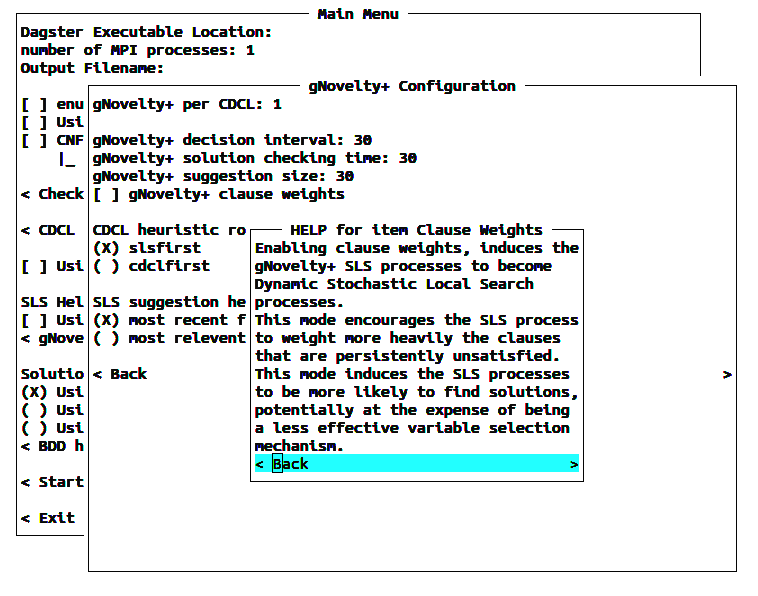
\includegraphics[width=0.85\textwidth]{figs/tui2.png}
\caption[The \dagster TUI configuration wizard interface]{The \dagster TUI configuration wizard interface. This demonstrates the description of the Dynamic Local Search option the user can select, for the local search helper processes. }\label{fig:tui_wizard}
\end{figure}


The TUI configuration interface must be run in an environment with an appropriate version of Python, with appropriate libraries installed (particularly the UrWid library), and can be initialised from the command:

\begin{Verbatim}[frame=single]
python ./wizard.py
\end{Verbatim}

This TUI configuration wizard allows a more user friendly way of beginning and configuring a \dagster\ run.

\subsection{Usability Feature: TUI Monitoring Interface}\label{sec:tui_monitoring}

We provide an new interface that allows users to monitor a \dagster\ run, and to assist in diagnosing any issue that might arise.
%%
\dagster\ emits log messages while it is running.
For example, logs can be to standard error (\textit{stderr}), standard output (\textit{stdout}) and/or to appropriate log files (as configured by Google Logging library (GLOG) environment variables).
%%
The verbosity of logging is defined by an environment variable (\texttt{GLOG\_v}), and the log messages hold many kinds of messages, such as: timing information, debugging hints, message counts, worker process status updates, and various possible error messages.
At verbosity $2$ or higher, the log messages are sufficient to give all the most relevant information about the progress of a run.
In principle, parsing these logs allows users to check on the health of a \dagster\ solution process, and allows inspection and diagnoses of bottlenecks, or of stalling between subproblem nodes of the DAG.
%%
However, scanning through log files to ascertain the overall state of the \dagster\ system dynamics is not a user friendly process.
Thus, a program to automate this task was seen to be desirable, and is now provided with the latest \dagster\ release.

In order to diagnose the overall state of the \dagster\ system progress in solving a problem, the most relevent information is about the progress of the workers in generating/processing the messages passed between DAG nodes.
The depiction of the DAG with messages flowing between nodes, and the progress workers have made on nodes, constitutes a summary of overall \dagster\ progress that is amenable to graphical representation.
For the reasoning as given in Section \ref{sec:tui_wizard}, we developed a separate graphical TUI module that parses the relevant log files, and pulls out the most relevant information for graphical display.
It is able to provide a graphical view of the DAG, along with statistics about worker progress and any relevant error messages.

A section of the TUI is shown in Figure \ref{fig:tui_monitoring}.
From this interface, we can see on the left hand side a text based graphical viewer of the DAG nodes, by their index, and the connections between them.
Next to that, we can see that there are three worker processes actively working on various DAG nodes.
Also rendered is the exact number of messages/solutions passed between each of the nodes of the DAG -- I.e., specifically the number of solutions ingested, completed, and output to subsequent nodes for processing.
%%
For each node, the TUI also reports the timing statistics for how long it takes for each worker process to complete a message,  including the average (and standard deviation) of seconds it takes to find one (or any) solutions for each of the messages, along with  how long it takes for workers to prove that there are no further messages before completing the message.
At the bottom of the TUI we render the miscellaneous log messages, which can be useful for error diagnosis.

Figure \ref{fig:tui_monitoring} depicts the interface when rendering runtime information related to the DAG shown in Figure \ref{fig:pentomino_dag_3x3}.
Here, Node 0 connects to Nodes 1 and 3, Node 1 connects to Nodes 2 and 4, etc.
The reader can see that there are three worker processes working concurrently on Nodes 1, 2 and 6.
Node 0 has fully completed one message inwards, and has completed giving 3 messages of output.
These output messages have been given to Nodes 1 and 3, with Node 3 taking one of these to produce an output message that has been given to Node 6 -- I.e., which is currently being worked upon, etc.
%%
Below this we can see an update from the worker logs, identifying themselves as working on Nodes 1,2 and 6.
The master process also periodically logs timing information related to workers on assigned nodes, the interface here reporting their performance when working on Nodes 1 and 3. 
%%
The TUI also renders a  Master health-status field, which is currently blank, indicating it is normal; and an `Exit' button.
%%
The 'unparsed' console message field will contain messages that have not been interpreted and rendered elsewhere in the TUI. Serious error messages will be rendered here, in case a serious error occurs.

We note that the DAG shown in Figure \ref{fig:pentomino_dag_3x3}, and the problem that is being run in this instance, as shown in Figure \ref{fig:tui_monitoring}, is actually a pentomino problem whose generation is explained in later Section \ref{sec:experiment_pentominos}.

The sequence of commands used to generate the screenshot shown in Figure \ref{fig:tui_monitoring} was as follows.
First, there was Google logging library (GLOG) environment variables specifying that it was to output logs to \textsc{stderr}, and at log level $3$.
\dagster\ was initialised with $4$ processes (1 master and 3 workers), and to pipe standard error to a file named `log\_output.txt':

\begin{Verbatim}[frame=single]
export GLOG_logtostderr=true
export GLOG_v=5
mpirun -n 4 ./dagster <DAG> <CNF> 2> log_output.txt
\end{Verbatim}

Secondly, in a separate shell, the following call was used to initialise the TUI monitoring program to parse the \dagster\ generated log file.

\begin{Verbatim}[frame=single]
python ./viewer.py <DAG> log_output.txt
\end{Verbatim}

The particular CNF and DAG file which was used was a pentomino problem generated as per Section \ref{sec:experiment_pentominos}, consisting of solving an 3x3 array of pentomino tiles.



The monitoring process allows a visualisation of how \dagster\ is progressing throughout the problem solution process.
However, the interface is primarily passive, consisting of monitoring the logs and outputting relevant information to the screen for users to see.
In order to change the way the \dagster\ program is running, pausing it and/or halting it, it is necessary to store the progress and/or potentially reinitialise the \dagster\ system with that progress established.
To do this, there is a necessity of being able to store the progress that \dagster\ has completed, via `checkpointing'.


\begin{figure}[h]
\centering
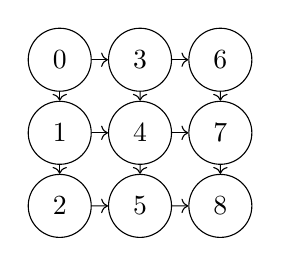
\begin{tikzpicture}[yscale=-0.91,scale=1.02]
	\node [fill=white, draw=black, shape=circle, minimum size=8mm] (0) at (0, 0) {0};
	\node [fill=white, draw=black, shape=circle, minimum size=8mm] (3) at (1, 0) {3};
	\node [fill=white, draw=black, shape=circle, minimum size=8mm] (6) at (2, 0) {6};
	
	\node [fill=white, draw=black, shape=circle, minimum size=8mm] (1) at (0, 1) {1};
	\node [fill=white, draw=black, shape=circle, minimum size=8mm] (4) at (1, 1) {4};
	\node [fill=white, draw=black, shape=circle, minimum size=8mm] (7) at (2, 1) {7};
	
	\node [fill=white, draw=black, shape=circle, minimum size=8mm] (2) at (0, 2) {2};
	\node [fill=white, draw=black, shape=circle, minimum size=8mm] (5) at (1, 2) {5};
	\node [fill=white, draw=black, shape=circle, minimum size=8mm] (8) at (2, 2) {8};
	
	\draw [fill=none, ->] (0) to (3);
	\draw [fill=none, ->] (0) to (1);
	\draw [fill=none, ->] (1) to (4);
	\draw [fill=none, ->] (1) to (2);
	\draw [fill=none, ->] (2) to (5);
	
	\draw [fill=none, ->] (3) to (6);
	\draw [fill=none, ->] (3) to (4);
	\draw [fill=none, ->] (4) to (7);
	\draw [fill=none, ->] (4) to (5);
	\draw [fill=none, ->] (5) to (8);
	
	\draw [fill=none, ->] (6) to (7);
	\draw [fill=none, ->] (7) to (8);
	
\end{tikzpicture}
\caption[DAG for a 3x3 pentomino superproblem]{DAG for a 3x3 pentomino superproblem - Decomposition A, further described in Section \ref{sec:experiment_pentominos}}\label{fig:pentomino_dag_3x3}
\end{figure}

\begin{figure}[h]
\centering
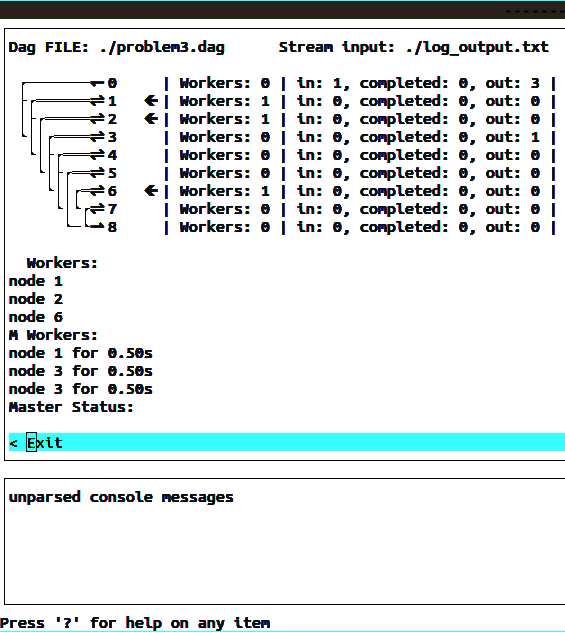
\includegraphics[width=0.85\textwidth]{figs/tui3.png}
\caption{The \dagster TUI monitoring interface}\label{fig:tui_monitoring}
\end{figure}


\FloatBarrier
\pagebreak
\subsection{Usability and Performance Feature: Checkpointing}\label{sec:checkpointing}

One primary design aspect of \dagster\ is the ability to initialise, monitor, and process hard and/or difficult SAT problems.
In the process of solving long-running SAT problems, the priorities for HPC usage can motivate the user to interrupt the \dagster\ run, also the system can potentially crash.
%%
This motivates the need for a backup functionality, which is coded in \dagster\ as a checkpoint functionality.
The checkpointing functionality allows \dagster\ to store its progress, thereby enabling reinitialisation from a checkpoint, as desired.

The checkpointing functionality is initialised in the Master process, as the master not only holds the details of what work needs to be (and has been) done, but is therefore also most able to have responsibility for monitoring and backing up (and/or reloading) that work.
%%
The checkpointing functionality of \dagster\ is optional, and configurable.
Master can be configured to dynamically format and dump all the relevant progress data to a series of custom files, with dumps occurring at equal time increments.
These files are written, and then periodically overwritten, in a round-robin fashion by \dagster, so that there always is a sequence of recent checkpoints of progress.
These checkpoints that \dagster\ produces can be then loaded back up into \dagster, from the command line, in the event that a search is interrupted to be later resumed.

The checkpoints hold all of the logical information relevant to a solution process, and are not tied to any specific configurations of the \dagster system.
In this way, a checkpoint generated on one system can be loaded into \dagster on a different system with a completely different configuration of search processes, and types of search.
%%Alternatively, it is possible to reload a \dagster checkpoint back into \dagster with a different configuration of settings, potentially speeding up a solution process without discarding existing progress.
The primary constraint on the flexibility of the checkpoint functionality, is that checkpoints generated when the Master is using BDD representation of system progress, are incompatible with checkpoints generated when Master process is using tables to represent messages and system progress - and vice versa.
This incompatibility arises because these two representations are fundamentally different, and not directly compatible.

The new checkpointing functionality is exposed by command line options, where the user is able to specify: {\em (i)}  where the checkpoint files are to be placed and named, {\em (ii)} how often checkpoint files should be generated (if at all), and {\em (iii)} what (if any) checkpoint file should be loaded on initialisation.%% are specifications provided to \dagster at boot by commandline.


\subsection{Performance Feature: \\Interface for Integrating Systematic Search Algorithms(e.g., CDCL)} %%Module CDCL interface: and integration of \textsc{MiniSAT}}
\label{sec:minisat_integration}

\dagster\ was originally built with all the CDCL worker processes implementing a systematic search based on
\textsc{TiniSAT}~\cite{huang2007tinisat,huang:and:veloso:2007}.
Modifications to the \textsc{TiniSAT} algorithm were made to support the interaction with local search processes, that  provide search guidance and solutions, and with possible strengthener processes that dynamically simplified \tinisat's learned clauses.
%%
%%However in much earlier versions of the \dagster\ system, before the integration of SLS and strengthener processes and interactions, the \dagster\ system was more modular and provided an interface for any CDCL solver to be integrated into \dagster\.
%%This modularity was eventually discarded with the interaction of these new elements.
%%
Recent experimentation with pentomino problems---see results in Section \ref{sec:experiment_pentominos}---motivated us to enable \dagster\ to more easily support different search algorithms.
For example, \tinisat\ is less effective than an alternative CDCL solver, namely \textsc{MiniSAT}~\cite{een2003extensible}, at pentomino problems. Therefore, being able to parametrically select to use  \textsc{MiniSAT}, rather than \textsc{TiniSAT}, as the base systematic search procedure is motivated. %%  it was hypothesized and then consequently proved that if \dagster\ was integrated with \textsc{MiniSAT} then there would be performance improvements.

\dagster\ was modified to incorporate \textsc{MiniSAT} as an option for the worker processes, and the modular interface implemented for these purposes can also support the integration of other CDCL solvers.
The modular interface more readily allows any CDCL solver to now be integrated with \dagster, by inheriting a virtual class in \textsc{C++} with appropriately overloaded methods.
In this way we anticipate that it should be easily possible to incorporate further CDCL solvers as options into the \dagster\ system.
We have yet to support all the integrations between subsolver types for such interactions, such as local search based guidance and strengthening of learnt clauses. 


\subsection{Performance Feature: Negative Literal Purging}\label{sec:negative_literal_purging}

Many SAT problems, and subproblems, feature solutions that are entirely (and immediately) derivable by an assignment over positive literals only.
%%
Such a fact is evident in our experiments, particularly the Costas and pentomino problems in Sections \ref{sec:experiment_costas} and \ref{sec:experiment_pentominos}, where the relevant information between subproblems consists entirely of where the points/pentominoes are, and thus from the positive literals in a solution valuation, all the negative information about where the points/pentominoes are not is then immediately implied.
%%
By having workers eliminate negative literals from solution records, the messages between processing elements can be greatly minimised.
In order to experiment and take advantage of this fact, we created a new \dagster\ mode for having workers purge negative literal information from messages and solution records.
In this way a lot of communication overhead in these problems is reduced, resulting in a material runtime performance enhancement. 

A consequence of this option is that \dagster\ is potentially unsound, because purging of negative variable information along the arcs of the DAG may mean a loss of solution information in specific problem cases where negative information is necessary.
%%
In principle, binary variables and their participation in a SAT problem can be coded negatively, or positively, just as effectively.
This new mode of operation effectively primes \dagster\ to take advantage of a particular bias in the way that people tend to code problems into SAT - particular that positive information is usually coded positively, and that negative variable evaluations are often consequences of that.

The unsafe purging just described was seen to be effective at improving solution times in pentomino problems (see Section~\ref{sec:experiment_pentominos}), however a safer alternative approach was sought.
Described next in Section~\ref{sec:literal_trimming}, an approach compliant with soundness and completeness is described, which is  computationally more expensive than the negative literal purging approach just described.
 

\subsection{Performance Feature: Literal Trimming}\label{sec:literal_trimming}

CDCL solvers by default (such as \tinisat\ and \textsc{MiniSAT}) report a valuation over all the variables when they find a satisfying valuation.
However, this full valuation is potentially overspecified, as a subset of those variables may be able to satisfy the CNF.
%%
For example, consider the CNF shown in Figure \ref{fig:example_cnf}.
The valuation $[1,-2,3,-4,5,6,7]$  solves this CNF, however there is redundancy as more variables are assigned than is necessary to satisfy the CNF.
%%
Specifically, the valuation $[1,3,5,6,7]$ satisfies the CNF without specifying the truth values of variables $2$ and $4$, and a shortened valuation such as this encompases a solution to the CNF with thoes variables specified any way. %%and therefore encompass the information that any of the four valuations of those variables is also a solution.
%%
In this way, the shorter the subproblem solutions encountered by \dagster\, the less work \dagster\ potentially has to do in enumerating the span of subproblem solutions.
Thus, with shorter valuations, \dagster\ is able to compute and record a smaller and more succinct representation of a set of solutions, thereby performing less search and using less system memory. 
%%
%%in enumerating all the satisfying solutions to a subproblem, and the less overspecified, the more solution space each message covers, and thus allows \dagster\ to enuemerate across possible solutions more effectively with fewer messages of shorter length.

The \dagster\ workers (optionally) implement a solution trimming procedure, where after a worker generates a solution to a given subproblem, it then analyses what variables can be removed from that solution such as to leave the SAT problem immediately satisfied irrespective of which way those trimmed variables would be assigned.
%In this way, a trimmed solution represents multiple solutions at once, and minimises the number and size of solutions communicated in the \dagster\ system, allowing more effective solving.
%
Previously, \dagster\ workers implemented a more rudimentary trimming system, eliminating all variables which were not present in the first satisfied variable of every CNF clause (considered in turn).
%%
%%Specifically,  every variable which was the first satisfied variable in every clause, and excluding any remainders.
To contrast the new approach with our historical trimming approach, consider the valuation $[1,-2,3,-4,5,6,7]$ to the problem in Figure~\ref{fig:example_cnf}.
%%
Previously, a \dagster\ worker would take the first clause, $(2\; 1\; 0)$, and conclude that $1$ must not be trimmed because it is the first literal that satisfies this first clause.
Then, that worker would take the second clause, $(-2\; 3\; 0)$, and conclude that $-2$ could not be trimmed because it was the first variable which satisfied the second clause.
The worker would continue thusly, concluding that the valuation $[1,-2,3,-4,5,7]$ was sufficiently trimmed with the only exclusion being the assignment to $6$.
%%
Our new trimming algorithm prioritises trimming of negative literals in a valuation, owing to the bias of human SAT encodings, that positive literals are generally more informative.
%%
With reference to the total valuation provided by the underlying search procedure, the new algorithm scans through each clause in turn, maintaining a monotonically increasing list of literals in the solution valuation it will report, as follows:%%, it would consider each clause in turn and:
\begin{enumerate}
\item	If the clause is not already satisfied by an element in the reporting list, then
\item	If there is a positive literal in the total valuation which satisfies the clause, then the worker adds the positive literal with the lowest absolute value to the reporting list.
\item	Otherwise, the worker adds the lowest absolute value indexed negative literal to the reporting list.
\end{enumerate}

After iterating over all clauses, only the literals in the reporting list are recorded as the discovered solution.
Continuing with the example from Figure~\ref{fig:example_cnf}, the run of this trimming algorithm,  given a total valuation $[1,-2,3,-4,5,6,7]$, would take the first clause $(2\; 1\; 0)$, and see that $1$ would be the lowest absolute value positive valuation in the solution to keep to satisfy the clause.
Processing the second clause, $(-2\; 3\; 0)$, and it finds that  $3$ is the smallest absolute value positive literal satisfying the clause, which also satisfies clause $(4\; 3\; 0)$.
For clause $(5\; -4\; 0)$, literal $5$ is added to the reporting list, etc.
%%
The reported solution by a worker is $[1,3,5,6,7]$, which is the total valuation excluding the assignments to the two variables $2$ and $4$.
It is both more effective as a trimming algorithm, and also has a direct bias towards keeping positively valued literals.

The optional inclusion of this trimming algorithm, is marginally more computationally expensive than the negative literal purging process described in Section~\ref{sec:negative_literal_purging}, but unlike that approach is provably sound and complete.


\begin{figure}
\begin{Verbatim}[frame=single, label=CNF file]
p cnf 7 6
2 1 0
-2 3 0
5 -4 0
4 3 0
4 -6 7 0
-4 6 0
\end{Verbatim}
\caption{An example CNF file}\label{fig:example_cnf}
\end{figure}

\subsection{Performance Feature: Geometric Restarting Strategy}\label{sec:dynamic_restarting}

The efficiency of systematic backtracking search to solve the SAT decision problem is premised on a restarting strategy~\cite{marques2021conflict}.
A backtracking decision procedure is said to restart when the current variable assignments being investigated are abandoned, and the search directed to start again with zero assignments made.
The benefit of restarting has been demonstrated theoretically, with restarting noted as the feature that enables a clause learning search to polynomially simulate the powerful general resolution procedure~\cite{pipatsrisawat:darwiche:2011,hertel:etal:2008,buss2021proof}.
In practice, mechanisms for restarting are also recognised as important~\cite{gomes:etal:1998,armin:hans:2008,audemard2012refining,biere2015evaluating}, with adaptive search policies characterised by restarting featuring in all performant algorithms. 
%%
The default CDCL algorithm implemented by \dagster\ systematic search processes---which is based on the {\textsc TiniSAT} algorithm---was indeed motivated by the recognition of the importance and the study of restarting~\cite{huang:2007}.
That base procedure offers a great deal of flexibility, regarding what restarting mechanisms researchers can implement, investigate and study.
We discuss a new restarting mechanism we have implemented in that default systematic search of \dagster.

Prior to describing our new restarting mechanism, it is worth motivating the need for our new approach.
When using \dagster\ to solve \#SAT problems, search processes use the same CDCL algorithm to drive both: {\em (i)}  model enumeration, and {\em (ii)} the exercise of proving that no further models exists -- i.e., performing an UNSAT proof, which is ideally done using a distinct restarting mechanism~\cite{oh2015between}.
We note that, even when the underlying \dagster\ query is to solve a SAT decision problem, and not a \#SAT counting problem, due to the compositional structure of the associated DAG the query can still pose subproblems that require subproblem model enumeration. 
Our new restarting mechanism adapts the frequency of restarting, so that when enumeration becomes difficult the search rapidly shifts towards an aggressive restarting approach that is relatively efficient at proving UNSAT.
We find that our dynamic approach dramatically improves the efficiency of proving UNSAT, and of discovering ``hard-to-find'' models in a counting problem.
Specifically, our new ``geometric'' restarting approach is very important for the best results we document for the Costas case study below.

With geometric restarting, the search implements restarts based on a dynamic probability-of-not-restarting (PnR) value.
Whenever a search discovers a new satisfying model to the subproblem it is assigned, the PnR value is set to its initial value, $1$.
Whenever $n$ conflicts are encountered,\footnote{Value $n$ is a hyperparameter set to $800$ by default.} the PnR is updated to be its current value multiplied by a discount factor $0 \leq \alpha <1$.\footnote{Value $\alpha$ is a hyperparameter set to $.95$ by default.}
Thus, if the search is not fruitful the probability of restarting approaches $1$, geometrically, and whenever the search yields a satisfying model this is reset to $0$.
Prior to the PnR being updated, a restart event is triggered with probability $\rho=(1 - \text{PnR})$.

To our knowledge we are the first to consider this dynamic restarting mechanism, and note that it is peculiar to our setting, where a systematic search is assigned to enumerate models to subformulae in the context of a larger monolithic search exercise.
Our new search mechanism is motivated to accelerate the enumeration process, and to free up search processes relatively quickly when no more subproblem models are available. 


\subsection{Performance Feature: Alternative Modes of Memory Operation}\label{sec:memory_operation}

\dagster\ takes a CNF and DAG file as input, specifying the problem and its decomposition respectively.
The system can then handle this CNF file in different ways depending on configuration.

Currently there are three configurations:
\begin{enumerate}
\item	The input CNF is loaded from file into the memory of every process, with all subproblems specified in the input DAG stored in memory.

  
\item	The input CNF is split into an array of CNF files, each corresponding to a subproblem from the input DAG. Workers only input and hold the CNF file of the subproblem they are working on.
  
\item	$\star$ {\textbf NEW}$\star$ The input CNF is scanned by all workers, with those storing only the clauses associated with the currently assigned subproblem.
  
\end{enumerate}

Each of these modes strikes a balance between computing speed, and memory requirements for larger CNF problem instances.
SAT problems in CNF can range from Kilobytes to Gigabytes, and when there are many workers each having copies and working on larger CNF subproblems, this can quickly exhaust the available memory.

For the smallest CNF files, it is most efficient to choose Option~1 of these configurations.
The whole CNF is loaded into the memory of every worker, and each worker does all possible preprocessing on their own copy of the CNF, involving splitting it into CNFs corresponding to all subproblems stored in memory.
In this way, each worker has maximal speed in directly accessing and manipulating its own local information in memory, involving the full and split problem CNFs.
Option~1 maximises speed, but comes at the cost of having a greater memory requirement for each worker process, and therefore the \dagster\ system overall.

For the very largest CNF files, it is better to use the Option~2 configuration, where at no point is the whole problem CNF itself ever loaded into memory, but the \dagster\ system leans on file storage for the storage and manipulation of CNF parts.
In this way CNF files potentially larger than the computer has memory can be handled and solved.
This configuration option is ideal for larger CNF files, but comes at the cost of having to load and reload CNF subproblem files as the \dagster\ run progresses, requiring greater amount of runtime consumed by file IO operations.

The new Option~3 configuration is a middle ground between the Options 1 and 2, where each worker parses and holds the original input CNF, but only the required target subproblem CNF is generated and stored in the worker's memory. In this way each worker operates in its own local memory space, but there is larger amount of IO and memory manipulation as the \dagster\ run progresses.



\subsection{Performance Feature: SLS Neighbourhood Calculations}\label{sec:neighbourhood_calculation}

Part of the startup process of the local search module, based on \gnoveltyp, is the process of calculating the sets of clauses connected to each variable, and the variables that are thereby neighbours in these clauses.
In the process of the SLS operation, variable values are flipped, and the scores associated with each of the variables are updated.
The score associated with a variable during search reflects the net number of clauses satisfied by a variable if it were to be flipped.
When a variable is flipped this causes some clauses to be satisfied and others to become unsatisfied, thus influencing the score of the flipped neighbourhood of the flipped variable.
%%
For this process of updating the score of variables that are induced by a flip of one of them, it is expedient for the computer to have a store of what variables are a neighbour of each other.
However, there are several issues creating this data store of variable neighbours, particularly as larger CNF files often feature several millions of variables, many of which may be neighbours of each other; and thus raw storage of this information can constitute Gigabytes of memory, consequently the process of calculating and/or accessing this information can become prohibitive.
%%
The creation of the variable neighbourhood data structure involves the insertion of many pairwise variable integers into a larger data set which preserves these pairs uniquely, and this information is then read many times over as the SLS progresses.
For this purpose there is a range of possible data structures which can can be employed, each with potential tradeoffs.
%%
The following functions are included in the \dagster\ project which outlay different ways of calculating variable neighbourhood information.
%We have implemented the following optimisations, related to the calculation and storage of neighbourhood information, which improve system performance over the tabular structures used in older versions of \dagster.

\pagebreak
\paragraph{Previous Implementation:}
\begin{enumerate}
\item Create an array with a Boolean flag for each variable.
\item Then iterate over all the variables, one by one:
\begin{itemize} 
\item Scan through the clauses in which the variable occurs, and for each of the variable's neighbours, set the neighbour's flag in the array to be true.
\item Scan through the array for all variables whose flag is set, to determine the neighbourhood of the variable, which is then stored more compactly as a static list.
\item Clear the array of flags
\end{itemize}
\end{enumerate}

This algorithm was previously implemented in the \dagster SLS routine, and while it is has constant insertion time (array look up and setting a flag), it also suffers from quadratic complexity in terms of the total number of variables, as each variable's neighbourhood is resolved by scanning over the array of flags, which has the size of the number of variables itself.
This quadratic complexity was seen to be an immediate bottleneck on larger problems.
However at the end of the algorithm, each variable has a static list of its neighbours, which is compact with a fast lookup.
%%
To ameliorate the issue of quadratic complexity in computation, we considered a different data structure to hold variable neighbourhood information, particularly we used the \textsc{C++} template library \textsc{set} to hold candidate variable neighbours and to purge duplicates, The first of two new implementations is as follows:

\paragraph{New Implementation 1:}
\begin{enumerate}
\item Then iterate over all the variables, one by one:
\begin{itemize} 
\item Initialise an empty \textsc{set} structure
\item For each clause in which the variable occurs, insert its neighbours into the set.
\item Scan through the set for all the neighbours of the variable, and then store the neighbours more compactly as a static list.
\end{itemize}
\end{enumerate}

This algorithm improves the quadratic complexity over total variables in the computation, with a logarithmic insertion cost (over the size of the set) throughout the iteration.
This logarithmic insertion cost is an inherent part of the \textsc{C++} standard template \textsc{set} structure, which stores and manipulates data in red-black trees.
This much improved algorithm made it possible to run \dagster's SLS modules with larger SAT problems, with many more variables.

Unfortunately it was noted that the memory consumption of the \textsc{set} datastructure, and the logarithmic calculation time became prohibitive on larger problem instances.
To remedy these observed problems, a second alternative algorithm was implemented, using duplicate data structure to improve speed and memory performance. The second new implementation is as follows:

\paragraph{New Implementation 2:}
\begin{enumerate}
\item Create an array with a Boolean flag for each variable.
\item Then iterate over all the variables, one by one:
\begin{itemize} 
\item Initialise an empty list structure
\item For each clause in which the variable occurs, and for each neighbour in that clause, check if the neighbours flag is set in the array, if it is not then set its flag, and add it to the list.
\item The list stores the  neighbourhood of the variable.
\item Clear the array of flags
\end{itemize}
\end{enumerate}

This implementation uses two data structures, a list and an array of flags, to hold neighbourhood information as it is being compiled, using the constant lookup time of the array of flags, to check uniqueness, and the list to store unique entries.
The neighbourhood information is compiled directly as a list which is then used in the SLS routine.
This implementation, uses linear operations for lookup, and insertion and compilation of information, without being as memory expensive as the \textsc{set} data structures.
Using this optimised implementation, the \dagster's SLS routine was able to work for larger SAT instances.


\section{Case Studies}\label{sec:casestudies}


In the previous sections we highlighted all the newer features and changes to \dagster since the last report deliverable.
The contributions include a range performance optimisations, new functionalities, operating modes, and user interfaces.
Using these feature additions, we were able to improve the runtime performance on several problems documented in the previous report, particularly Costas array counting and pentomino problems.
In these case studies, some of the features which we introduced proved to be useful in providing performance gains relative to other solvers.
%%
A range of other solvers were newly considered as performance comparisons against \dagster.
These performance comparisons are primarily shown in Figures \ref{fig:costas_performance2} and \ref{fig:performance_graph46461}.
%%
In addition to extending these two familiar case studies, we also introduce a new case study not included in the previous report, particularly using \dagster\ in Bounded Model Checking (BMC) between different variable fidelities using abstraction invariant variable values.
%In this new case study, we coded in \textsc{C} a bidirectional communication protocol and used CMBC to generate SAT CNF files.
%The encoding was computed multiple times, each time using  different bit fidelities for the variables of the encoding.
%We show that, using \dagster, the solutions to low fidelity compiled models can be communicated to subprocesses working on higher fidelity models, minimising the overall number of decisions needed to be made by the \dagster\ procedure to compute a solution to the highest fidelity, which corresponds to a faithful model of the underlying problem. %% abstraction invariant control flow variable values from lower fidelity models can be translated to the higher fidelity models yielding improved runtime performance, as we shall see.

We consider three case studies:
\begin{itemize}
\item	In Section \ref{sec:experiment_costas}, we consider performance in parallel model counting of Costas arrays, contrasting \dagster\ performance against the state-of-the-art \textsc{DMC} parallel model counter, showing performance enhancement due to geometric restarting, and SLS \& Strengthener integration.
  
\item	In Section \ref{sec:experiment_pentominos}, we consider performance in solving generated pentomino problems, showing the performance enhancement provided by different decompositions, and the choice of \dagster's underlying CDCL solver against a wider range of state-of-the-art distributed and parallel SAT tools.
  
\item In Section \ref{sec:mc:bmc}, we show the performance enhancement in a  BMC case study, using \dagster's decomposition approach to carry abstraction invariant variable values between variable-fidelity models.
\end{itemize}

\pagebreak
\subsection{Costas Arrays}\label{sec:experiment_costas}

\paragraph{New features} of \dagster\ that are being used when generating the experimental data reported on for this case study are: {\em (i)} new efficient search neighbourhood representations as described in Section~\ref{sec:neighbourhood_calculation}, {\em (ii)} in Table~\ref{fig:costas_data_table} specifically, the reported runtime data is gathered with \dagster\ using the geometric restarting policy described in Section~\ref{sec:dynamic_restarting}, and {\em (iii)} we use the sound and complete approach to trimming solution literals described in Section~\ref{sec:literal_trimming}. $\qed$\\\rule{50pt}{5pt}


A Costas array is a set of $n$ points in an $n\times n$ array such that each column and row contains exactly one point, and each of the $n(n-1)/2$ displacement vectors between the points are distinct.
An example Costas array is shown in Figure~\ref{fig:costas1}. 
%%
Using search to solve for Costas arrays is known to be challenging, and searching processes have been conducted at least up to size $n=29$~\cite{DBLP:journals/amco/DrakakisIRW11,darakakis:etal:2008}.
However, whether arrays exist at $n\in\{32,33\}$ is an open problem.
As a number of Costas array subclasses at those sizes have been eliminated~\cite{748721}, it is conjectured (but not confirmed) that Costas arrays of those sizes do not exist~\cite{conf/ciss/RussoEB10}.





\begin{figure}[b]
%\captionsetup[subfigure]{justification=centering}
\centering


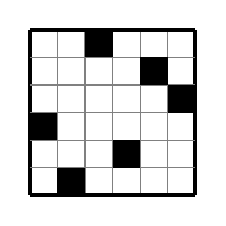
\begin{tikzpicture}[xscale=0.35, yscale=-0.35]
\draw[ultra thick] (0,0)--(0,6);
\draw[gray,thin] (1,0)--(1,6);
\draw[gray,thin] (2,0)--(2,6);
\draw[gray,thin] (3,0)--(3,6);
\draw[gray,thin] (4,0)--(4,6);
\draw[gray,thin] (5,0)--(5,6);
\draw[ultra thick] (6,0)--(6,6);

\draw[ultra thick] (0,0)--(6,0);
\draw[gray,thin] (0,1)--(6,1);
\draw[gray,thin] (0,2)--(6,2);
\draw[gray,thin] (0,3)--(6,3);
\draw[gray,thin] (0,4)--(6,4);
\draw[gray,thin] (0,5)--(6,5);
\draw[ultra thick] (0,6)--(6,6);

\fill [black] (2,0) rectangle (3,1);
\fill [black] (4,1) rectangle (5,2);
\fill [black] (5,2) rectangle (6,3);
\fill [black] (0,3) rectangle (1,4);
\fill [black] (3,4) rectangle (4,5);
\fill [black] (1,5) rectangle (2,6);

\end{tikzpicture}
%\caption{Costas array for $n=6$.}\label{fig:costas1}

\caption{An example Costas array}\label{fig:costas1}


\end{figure}


\begin{figure}[t]
\centering

%\vspace{-1cm}

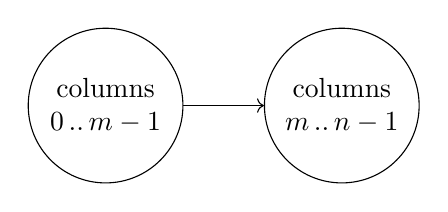
\begin{tikzpicture}
	\node [fill=white, draw=black, shape=circle, text width=1.5cm, text centered] (0) at (0, 0) {columns $0\, .. \, m-1$};
	\node [fill=white, draw=black, shape=circle, text width=1.5cm, text centered] (1) at (3, 0) {columns $m\, .. \, n-1$};
	\draw [fill=none, ->] (0) to (1);
\end{tikzpicture}
%\caption{DAG for Costas problem.}\label{fig:dag_example121}

\caption{A DAG decomposing Costas problem into two parts.}\label{fig:dag_example121}


%\caption{An example Costas array, and a DAG decomposing Costas problem into two parts.}\label{fig:costas_subfigure}\label{fig:dag_example121}\label{fig:costas1}
\end{figure}


For each size $n$, we can directly synthesise a CNF formula whose models are in one-to-one correspondence with the set of Costas arrays of size $n$, and Lex-leader constraints can be added to break the dihedral group symmetries (reflection and rotation) \cite{10.1007/11889205_46}.
For the purpose of using SAT-search to count unique arrays for values of $n$ using \dagster,  we employ a simple DAG structure, Figure \ref{fig:dag_example121}, with two connected vertices. The first node is the placing of the first $m$ columns of the Costas array, and the second part is the placement of the remainder.


The performance of \dagster at solving Costas problems for different sized Costas arrays $n$, and for different numbers of columns $m$ solved in the first node, for different numbers of cores and \dagster modes, is given in Figure~\ref{fig:costas_performance2}.
Here, we also compare \dagster\ against the distributed model counter \textsc{DMC}~\cite{lagniez:etal:2018}, and against the performance of model counting by repeatedly calling \tinisat. 
This figure shows the runtime results of including clause strengthening and/or local search helper processes, and also shows the effect of two different decompositions on the performance of Costas model counting.


%\input{figs/computing_times_GADI1.tex}

   \begin{figure*}[h]
        \centering
		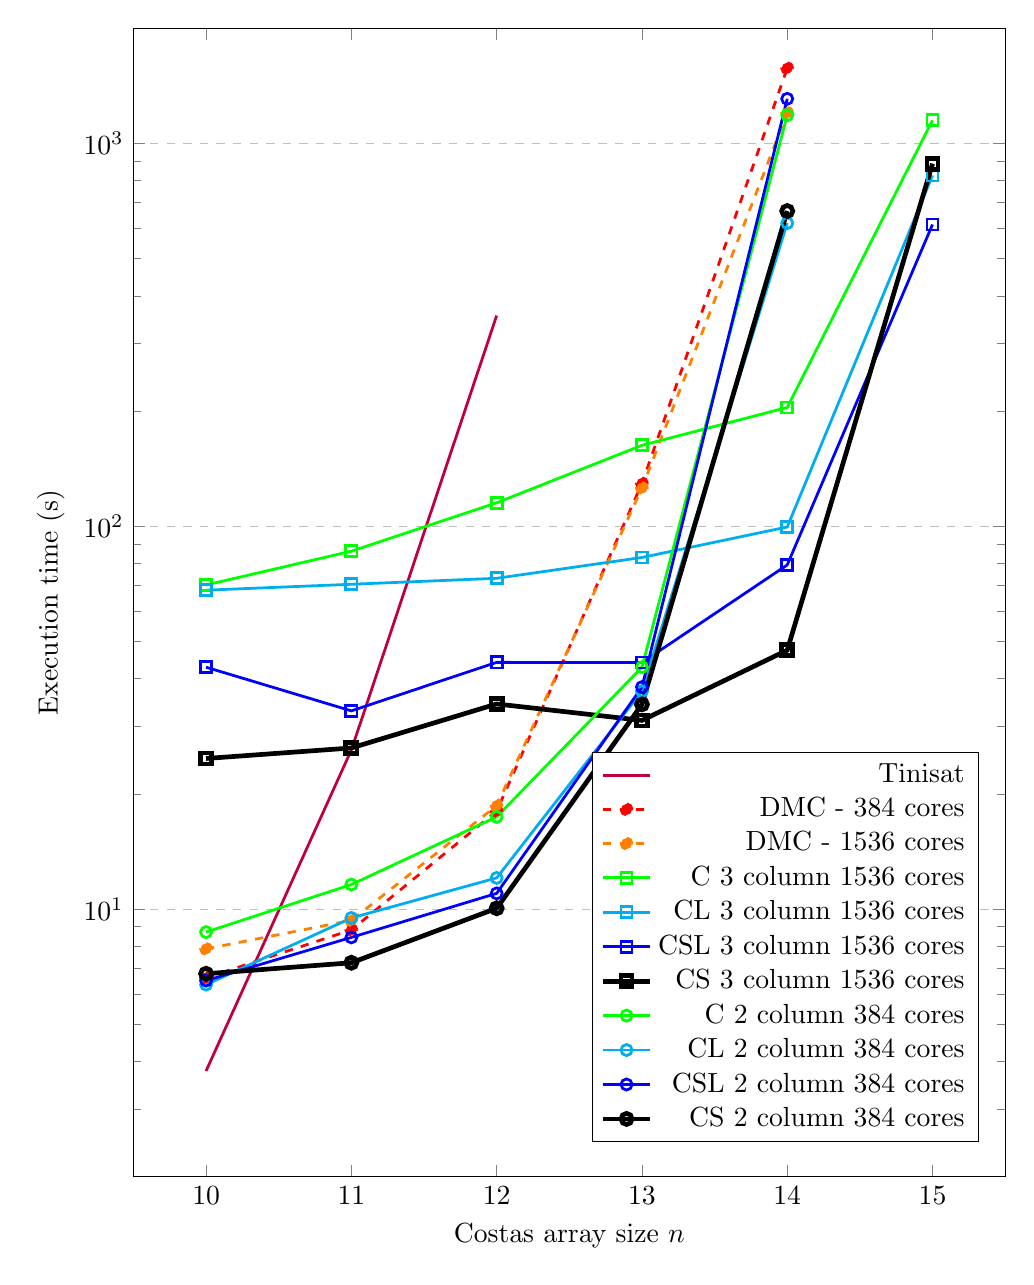
\begin{tikzpicture}
		\begin{axis}[
			title={},
			xlabel={Costas array size $n$},
			ylabel={Execution time (s)},
			%xmin=0, xmax=0.25,
			ymin=2.00, ymax=2000.00,
			ymode=log,
			xtick={10,11,12,13,14,15},
			%ytick={0,20,40,60,80,100},
			%yticklabel=$\pgfmathprintnumber{\tick}\%$,
			legend pos=south east,
			legend cell align=right,
			ymajorgrids=true,
			grid style=dashed,
			xticklabel style={/pgf/number format/fixed},
			width = 360,
			height = 460
		]




\addplot[color=purple,line width=1.0pt] coordinates {
(10,3.7782273292541504)(11,26.04908299446106)(12,355.1301419734955)}node[pos=0.8](endofplotsquare){} ;
\addlegendentry{Tinisat}




%\addplot[mark = diamond,color=green,line %width=1.0pt,dashed] coordinates {
%(10, 2.4890098571777344)
%(11, 15.25694990158081)
%(12, 149.58365178108215)
%(13, 2073.277750492096)
%(14, 3001.0201098918915)
%(15, 3001.0185282230377)
%(16, 3001.017208814621)
%(17, 3001.0177602767944)
%}node[pos=0.8](endofplotsquare){} ;
%\addlegendentry{DMC - laptop}


\addplot[mark = *,color=red,line width=1.0pt,dashed] coordinates {
(10, 6.614523410797119)
(11, 8.821394920349121)
(12, 18.032766580581665)
(13, 129.34079885482788)
(14, 1572.7557713985443)
%(15, 3004.0578289031982)
}node[pos=0.8](endofplotsquare){} ;
\addlegendentry{DMC - 384 cores}


\addplot[mark = *,color=orange,line width=1.0pt,dashed] coordinates {
(10, 7.872957944869995)
(11, 9.344036340713501)
(12, 18.633763074874878)
(13, 125.84372735023499)
(14, 1201.838926076889)
}node[pos=0.8](endofplotsquare){} ;
\addlegendentry{DMC - 1536 cores}






%\addplot[color=black,line width=0.8pt,dotted] coordinates {
%(10,268.601)
%(11,409.919)
%(12,612.876)
%(13,965.892)
%(14,1624.668)
%}node[pos=0.8](endofplotsquare){} ;
%\addlegendentry{\modezero 4 column 1536 cores}


\addplot[mark = square,color=green,line width=1.0pt] coordinates {
(10,70.254)
(11,86.081)
(12,115.172)
(13,162.719)
(14,204.369)
(15,1150.111)
}node[pos=0.8](endofplotsquare){} ;
\addlegendentry{\modezero 3 column 1536 cores}

\addplot[mark = square,color=cyan,line width=1.0pt] coordinates {
(10,68.087)
(11,70.551)
(12,73.140)
(13,82.886)
(14,99.570)
(15,824.921)
}node[pos=0.8](endofplotsquare){} ;
\addlegendentry{\modeone 3 column 1536 cores}


\addplot[mark = square,color=blue,line width=1.0pt] coordinates {
(10,42.836)
(11,32.946)
(12,44.104)
(13,44.056)
(14,79.275)
(15,614.229)
}node[pos=0.8](endofplotsquare){} ;
\addlegendentry{\modethree 3 column 1536 cores}

\addplot[mark = square,color=black,line width=1.7pt] coordinates {
(10,24.741)
(11,26.357)
(12,34.344)
(13,31.114)
(14,47.458)
(15,885.323)
}node[pos=0.8](endofplotsquare){} ;
\addlegendentry{\modetwo 3 column 1536 cores}





\addplot[mark = o,color=green,line width=1.0pt] coordinates {
(10,8.709)(11,11.592)(12,17.416)(13,42.837)(14,1185.395)
}node[pos=0.8](endofplotsquare){} ;
\addlegendentry{\modezero 2 column 384 cores}

\addplot[mark = o,color=cyan,line width=1.0pt] coordinates {
(10,6.349)(11,9.481)(12,12.062)(13,37.085)(14,619.429)
}node[pos=0.8](endofplotsquare){} ;
\addlegendentry{\modeone 2 column 384 cores}


\addplot[mark = o,color=blue,line width=1.0pt] coordinates {
(10,6.506)(11,8.435)(12,10.991)(13,38.013)(14,1308.012)
}node[pos=0.8](endofplotsquare){} ;
\addlegendentry{\modethree 2 column 384 cores}

\addplot[mark = o,color=black,line width=1.7pt] coordinates {
(10,6.779)(11,7.242)(12,10.048)(13,34.258)(14,665.972)
}node[pos=0.8](endofplotsquare){} ;
\addlegendentry{\modetwo 2 column 384 cores}




		\end{axis}
		\end{tikzpicture}
		%\vspace{-18pt}
		\caption[Runtime performance for Costas problems]{Runtime performance of \dagster\ against model counting with \tinisat\ and \textsc{DMC} on  Costas problems with different number of columns in the decomposition and processor cores. \modezero = CDCL only; \modeone = CDCL + local search; \modetwo = CDCL + strengthener; \modethree = CDCL + strengthener + local search; \dagster\ running with \tinisat CDCL core. One local search process per worker group.}
		\label{fig:costas_performance2}
    \end{figure*}


In these figures, the time taken to count all the Costas arrays of a given size is plotted, and we can see that for larger sized Costas arrays, \dagster\ is significantly faster than \tinisat\ at solving the Costas model counting problem, and that performance can be improved further using \dagster's additional feature modes.
For smaller and easier Costas problems (of size $n\le 12$) the parallel overhead of using \dagster\ is the primary determinant of the solution time, and \dagster\ performs worse than \tinisat which has minimal overhead; this overhead is most pronounced with the more granular decompositions that include more columns (e.g. for Costas-10, 3-column is worse than 2-column).
However, for larger and harder Costas problems ($n>12$), it is seen that \dagster consistently outperforms \tinisat\ - the CDCL procedure which \dagster is employing; as well as outperforming the \textsc{DMC} model counter.
Additionally, for large problems, having one local search (modes denoted with `L') and/or clause strengthening process (modes denoted with `S') per worker group complements the CDCL procedure to yield improved runtime.%, allowing larger Costas arrays to be computed more efficiently.

Another advantage of using \dagster\ is that it allows easy experimentation about the decomposition employed. In our results, we have considered decomposition into contiguous blocks of columns (where the first node has the first $m$ columns, and the second node has the remainder), but we can also consider decompositions with interleaved columns.
There are also many configurable variables related to restarting policy and variable selection controls.
In particular, we considered a vanilla VSIDS heuristic \cite{DBLP:conf/dac/MoskewiczMZZM01} and a fixed geometrically increasing restart policy (as introduced in Section \ref{sec:dynamic_restarting}).
In Table~\ref{fig:costas_data_table}, we can see how changing the index of the columns that \dagster\ decomposes the problem by can increase the runtime performance.



\begin{table}
\centering

\begin{tabular}{|l|l|l|l|l|}
\hline
Size (n) & Cores & Columns & S & Runtimes  \\ \hline
9 & 48 & \{4\} & & 5.527  \\ \hline
 10 & 2 & \{2,4\} & & 1.356  \\ \hline
10 & 48 & \{2,4\} & & 5.191  \\ \hline
11 & 2 & \{2,4\} & & 4.155  \\ \hline
11 & 48 & \{2,4\} & & 5.642  \\ \hline
12 & 48 & \{2,4\} & & 21.234  \\ \hline
12 & 48 & \{2,4\} & & 7.267  \\ \hline
12 & 48 & \{2,4\} & \checkmark & 7.419  \\ \hline
13 & 2 & \{2,4,6\} & & 91.22  \\ \hline
13 & 48 & \{2,4,6\} & & 8.427  \\ \hline
13 & 48 & \{2,4,6\} & \checkmark & 10.242  \\ \hline
14 & 2 & \{5,7,9\} & & 524.414  \\ \hline
14 & 384 & \{5,7,9\} & & 16.562  \\ \hline
14 & 383 & \{5,7,9\} & \checkmark & 12.118  \\ \hline
15 & 384 & \{5,7,9,11\} & & 118.133  \\ \hline
15 & 383 & \{5,7,9,11\} & \checkmark & 86.125  \\ \hline
16 & 528 & \{5,7,9,11\} & & 275.127  \\ \hline
16 & 527 & \{5,7,9,11\} & \checkmark & 235.25  \\ \hline
\end{tabular}


\vspace{4mm}
\caption[Costas problem table of runtime values]{Runtimes for different Costas problems with decompositions with columns in the first DAG node, with and without Strengthener (S) - i.e. modes \modezero and \modetwo (w/ \tinisat\ cores); runtime in seconds, against cores and sizes. }\label{fig:costas_data_table}
\end{table}


\FloatBarrier
\pagebreak
\subsection{Pentominoes}\label{sec:experiment_pentominos}

\paragraph{New features} of \dagster\ that are being used when generating the experimental data reported on for this case study are: {\em (i)}  we use the sound and complete approach to trimming solution literals described in Section~\ref{sec:literal_trimming}, and {\em (ii)} we contrast the runtime performance of \dagster\ using the systematic search algorithm based on {\textsc TiniSAT} with the performance using the algorithms from {\textsc MiniSAT}, thus using the new search interface described in Section~\ref{sec:minisat_integration}. $\qed$\\\rule{50pt}{5pt}

\input{figs/pentomino_puzzle.tex}





\begin{figure}[]
\centering


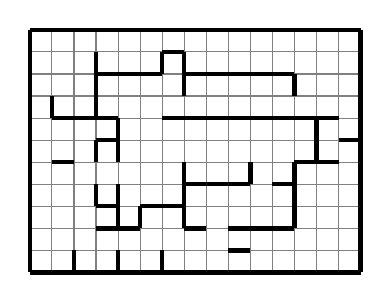
\begin{tikzpicture}[xscale=0.28, yscale=-0.28, rotate=0]
\draw[gray,thin] (0,0)--(0,11);
\draw[gray,thin] (1,0)--(1,11);
\draw[gray,thin] (2,0)--(2,11);
\draw[gray,thin] (3,0)--(3,11);
\draw[gray,thin] (4,0)--(4,11);
\draw[gray,thin] (5,0)--(5,11);
\draw[gray,thin] (6,0)--(6,11);
\draw[gray,thin] (7,0)--(7,11);
\draw[gray,thin] (8,0)--(8,11);
\draw[gray,thin] (9,0)--(9,11);
\draw[gray,thin] (10,0)--(10,11);
\draw[gray,thin] (11,0)--(11,11);
\draw[gray,thin] (12,0)--(12,11);
\draw[gray,thin] (13,0)--(13,11);
\draw[gray,thin] (14,0)--(14,11);
\draw[gray,thin] (0,0)--(15,0);
\draw[gray,thin] (0,1)--(15,1);
\draw[gray,thin] (0,2)--(15,2);
\draw[gray,thin] (0,3)--(15,3);
\draw[gray,thin] (0,4)--(15,4);
\draw[gray,thin] (0,5)--(15,5);
\draw[gray,thin] (0,6)--(15,6);
\draw[gray,thin] (0,7)--(15,7);
\draw[gray,thin] (0,8)--(15,8);
\draw[gray,thin] (0,9)--(15,9);
\draw[gray,thin] (0,10)--(15,10);
\draw[ultra thick] (6,1)--(7,1);
\draw[ultra thick] (3,1)--(3,2);
\draw[ultra thick] (3,2)--(4,2);
\draw[ultra thick] (4,2)--(5,2);
\draw[ultra thick] (6,1)--(6,2);
\draw[ultra thick] (5,2)--(6,2);
\draw[ultra thick] (7,1)--(7,2);
\draw[ultra thick] (7,2)--(8,2);
\draw[ultra thick] (8,2)--(9,2);
\draw[ultra thick] (9,2)--(10,2);
\draw[ultra thick] (10,2)--(11,2);
\draw[ultra thick] (11,2)--(12,2);
\draw[ultra thick] (3,2)--(3,3);
\draw[ultra thick] (7,2)--(7,3);
\draw[ultra thick] (12,2)--(12,3);
\draw[ultra thick] (1,3)--(1,4);
\draw[ultra thick] (1,4)--(2,4);
\draw[ultra thick] (3,3)--(3,4);
\draw[ultra thick] (2,4)--(3,4);
\draw[ultra thick] (3,4)--(4,4);
\draw[ultra thick] (6,4)--(7,4);
\draw[ultra thick] (7,4)--(8,4);
\draw[ultra thick] (8,4)--(9,4);
\draw[ultra thick] (9,4)--(10,4);
\draw[ultra thick] (10,4)--(11,4);
\draw[ultra thick] (11,4)--(12,4);
\draw[ultra thick] (12,4)--(13,4);
\draw[ultra thick] (13,4)--(14,4);
\draw[ultra thick] (4,4)--(4,5);
\draw[ultra thick] (3,5)--(4,5);
\draw[ultra thick] (13,4)--(13,5);
\draw[ultra thick] (14,5)--(15,5);
\draw[ultra thick] (1,6)--(2,6);
\draw[ultra thick] (3,5)--(3,6);
\draw[ultra thick] (4,5)--(4,6);
\draw[ultra thick] (13,5)--(13,6);
\draw[ultra thick] (12,6)--(13,6);
\draw[ultra thick] (13,6)--(14,6);
\draw[ultra thick] (7,6)--(7,7);
\draw[ultra thick] (7,7)--(8,7);
\draw[ultra thick] (8,7)--(9,7);
\draw[ultra thick] (10,6)--(10,7);
\draw[ultra thick] (9,7)--(10,7);
\draw[ultra thick] (12,6)--(12,7);
\draw[ultra thick] (11,7)--(12,7);
\draw[ultra thick] (3,7)--(3,8);
\draw[ultra thick] (4,7)--(4,8);
\draw[ultra thick] (3,8)--(4,8);
\draw[ultra thick] (5,8)--(6,8);
\draw[ultra thick] (7,7)--(7,8);
\draw[ultra thick] (6,8)--(7,8);
\draw[ultra thick] (12,7)--(12,8);
\draw[ultra thick] (4,8)--(4,9);
\draw[ultra thick] (3,9)--(4,9);
\draw[ultra thick] (5,8)--(5,9);
\draw[ultra thick] (4,9)--(5,9);
\draw[ultra thick] (7,8)--(7,9);
\draw[ultra thick] (7,9)--(8,9);
\draw[ultra thick] (9,9)--(10,9);
\draw[ultra thick] (10,9)--(11,9);
\draw[ultra thick] (12,8)--(12,9);
\draw[ultra thick] (11,9)--(12,9);
\draw[ultra thick] (9,10)--(10,10);
\draw[ultra thick] (2,10)--(2,11);
\draw[ultra thick] (4,10)--(4,11);
\draw[ultra thick] (6,10)--(6,11);
\draw[ultra thick] (0,0)--(0,11);
\draw[ultra thick] (0,0)--(15,0);
\draw[ultra thick] (15,11)--(0,11);
\draw[ultra thick] (15,11)--(15,0);
\end{tikzpicture}
\caption[An example Pentomino puzzle]{Pentomino puzzle featured on Youtube channel \emph{Cracking the Cryptic}~\protect\footnotemark}\label{fig:pentomino_puzzle1}



\end{figure}






\begin{figure}[tbp]
\hspace{1.5cm}%
\subfloat[][DAG for a 4x4 pentomino superproblem - Decomposition A]{
\centering
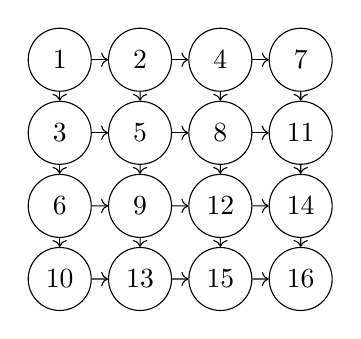
\begin{tikzpicture}[yscale=-0.91,scale=1.02]
	\node [fill=white, draw=black, shape=circle, minimum size=8mm] (1) at (0, 0) {1};
	\node [fill=white, draw=black, shape=circle, minimum size=8mm] (2) at (1, 0) {2};
	\node [fill=white, draw=black, shape=circle, minimum size=8mm] (4) at (2, 0) {4};
	\node [fill=white, draw=black, shape=circle, minimum size=8mm] (7) at (3, 0) {7};
	
	\node [fill=white, draw=black, shape=circle, minimum size=8mm] (3) at (0, 1) {3};
	\node [fill=white, draw=black, shape=circle, minimum size=8mm] (5) at (1, 1) {5};
	\node [fill=white, draw=black, shape=circle, minimum size=8mm] (8) at (2, 1) {8};
	\node [fill=white, draw=black, shape=circle, minimum size=8mm] (11) at (3, 1) {11};
	
	\node [fill=white, draw=black, shape=circle, minimum size=8mm] (6) at (0, 2) {6};
	\node [fill=white, draw=black, shape=circle, minimum size=8mm] (9) at (1, 2) {9};
	\node [fill=white, draw=black, shape=circle, minimum size=8mm] (12) at (2, 2) {12};
	\node [fill=white, draw=black, shape=circle, minimum size=8mm] (14) at (3, 2) {14};
	
	\node [fill=white, draw=black, shape=circle, minimum size=8mm] (10) at (0, 3) {10};
	\node [fill=white, draw=black, shape=circle, minimum size=8mm] (13) at (1, 3) {13};
	\node [fill=white, draw=black, shape=circle, minimum size=8mm] (15) at (2, 3) {15};
	\node [fill=white, draw=black, shape=circle, minimum size=8mm] (16) at (3, 3) {16};
	
	\draw [fill=none, ->] (1) to (3);
	\draw [fill=none, ->] (2) to (5);
	\draw [fill=none, ->] (4) to (8);
	\draw [fill=none, ->] (7) to (11);
	
	\draw [fill=none, ->] (3) to (6);
	\draw [fill=none, ->] (5) to (9);
	\draw [fill=none, ->] (8) to (12);
	\draw [fill=none, ->] (11) to (14);
	
	\draw [fill=none, ->] (6) to (10);
	\draw [fill=none, ->] (9) to (13);
	\draw [fill=none, ->] (12) to (15);
	\draw [fill=none, ->] (14) to (16);
	
	\draw [fill=none, ->] (1) to (2);
	\draw [fill=none, ->] (2) to (4);
	\draw [fill=none, ->] (4) to (7);
	
	\draw [fill=none, ->] (3) to (5);
	\draw [fill=none, ->] (5) to (8);
	\draw [fill=none, ->] (8) to (11);
	
	\draw [fill=none, ->] (6) to (9);
	\draw [fill=none, ->] (9) to (12);
	\draw [fill=none, ->] (12) to (14);
	
	\draw [fill=none, ->] (10) to (13);
	\draw [fill=none, ->] (13) to (15);
	\draw [fill=none, ->] (15) to (16);
\end{tikzpicture}
\label{fig:dag_example1215}
}\hspace{1.5cm}%
\subfloat[18cm][DAG for a 4x4 pentomino superproblem - Decomposition B]{
\centering
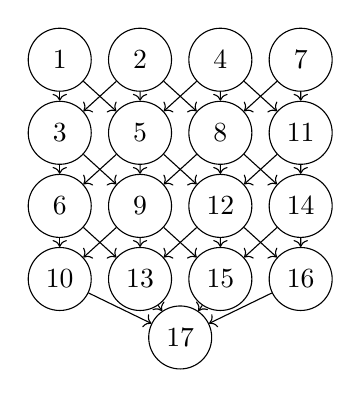
\begin{tikzpicture}[yscale=-0.91,scale=1.02]
	\node [fill=white, draw=black, shape=circle, minimum size=8mm] (1) at (0, 0) {1};
	\node [fill=white, draw=black, shape=circle, minimum size=8mm] (2) at (1, 0) {2};
	\node [fill=white, draw=black, shape=circle, minimum size=8mm] (4) at (2, 0) {4};
	\node [fill=white, draw=black, shape=circle, minimum size=8mm] (7) at (3, 0) {7};
	
	\node [fill=white, draw=black, shape=circle, minimum size=8mm] (3) at (0, 1) {3};
	\node [fill=white, draw=black, shape=circle, minimum size=8mm] (5) at (1, 1) {5};
	\node [fill=white, draw=black, shape=circle, minimum size=8mm] (8) at (2, 1) {8};
	\node [fill=white, draw=black, shape=circle, minimum size=8mm] (11) at (3, 1) {11};
	
	\node [fill=white, draw=black, shape=circle, minimum size=8mm] (6) at (0, 2) {6};
	\node [fill=white, draw=black, shape=circle, minimum size=8mm] (9) at (1, 2) {9};
	\node [fill=white, draw=black, shape=circle, minimum size=8mm] (12) at (2, 2) {12};
	\node [fill=white, draw=black, shape=circle, minimum size=8mm] (14) at (3, 2) {14};
	
	\node [fill=white, draw=black, shape=circle, minimum size=8mm] (10) at (0, 3) {10};
	\node [fill=white, draw=black, shape=circle, minimum size=8mm] (13) at (1, 3) {13};
	\node [fill=white, draw=black, shape=circle, minimum size=8mm] (15) at (2, 3) {15};
	\node [fill=white, draw=black, shape=circle, minimum size=8mm] (16) at (3, 3) {16};
	
	\node [fill=white, draw=black, shape=circle, minimum size=8mm] (17) at (1.5, 3.8) {17};
	
	\draw [fill=none, ->] (1) to (3);
	\draw [fill=none, ->] (2) to (5);
	\draw [fill=none, ->] (4) to (8);
	\draw [fill=none, ->] (7) to (11);
	
	\draw [fill=none, ->] (3) to (6);
	\draw [fill=none, ->] (5) to (9);
	\draw [fill=none, ->] (8) to (12);
	\draw [fill=none, ->] (11) to (14);
	
	\draw [fill=none, ->] (6) to (10);
	\draw [fill=none, ->] (9) to (13);
	\draw [fill=none, ->] (12) to (15);
	\draw [fill=none, ->] (14) to (16);
	
	\draw [fill=none, ->] (1) to (5);
	\draw [fill=none, ->] (2) to (8);
	\draw [fill=none, ->] (4) to (11);
	
	\draw [fill=none, ->] (3) to (9);
	\draw [fill=none, ->] (5) to (12);
	\draw [fill=none, ->] (8) to (14);
	
	\draw [fill=none, ->] (6) to (13);
	\draw [fill=none, ->] (9) to (15);
	\draw [fill=none, ->] (12) to (16);
	
	\draw [fill=none, ->] (2) to (3);
	\draw [fill=none, ->] (4) to (5);
	\draw [fill=none, ->] (7) to (8);
	
	\draw [fill=none, ->] (5) to (6);
	\draw [fill=none, ->] (8) to (9);
	\draw [fill=none, ->] (11) to (12);
	
	\draw [fill=none, ->] (9) to (10);
	\draw [fill=none, ->] (12) to (13);
	\draw [fill=none, ->] (14) to (15);
	
	\draw [fill=none, ->] (10) to (17);
	\draw [fill=none, ->] (13) to (17);
	\draw [fill=none, ->] (15) to (17);
	\draw [fill=none, ->] (16) to (17);
\end{tikzpicture}
\label{fig:dag_example1216}
}




\caption[Two possible DAG arrangements for Pentomino problems]{Two DAG arrangements for solving a cascaded grid of connected sub-problems}\label{fig:pentominos_subfigure}
\end{figure}








\footnotetext{\url{youtube.com/watch?v=S2aN-s3hG6Y}}

%\begin{figure}[h]
\centering
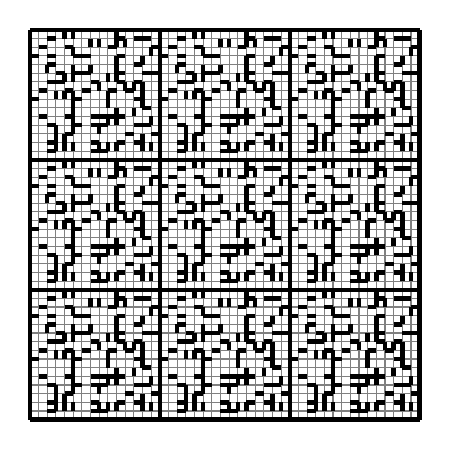
\begin{tikzpicture}[scale=0.11]
\draw[gray,thin] (0,0)--(0,45);
\draw[gray,thin] (1,0)--(1,45);
\draw[gray,thin] (2,0)--(2,45);
\draw[gray,thin] (3,0)--(3,45);
\draw[gray,thin] (4,0)--(4,45);
\draw[gray,thin] (5,0)--(5,45);
\draw[gray,thin] (6,0)--(6,45);
\draw[gray,thin] (7,0)--(7,45);
\draw[gray,thin] (8,0)--(8,45);
\draw[gray,thin] (9,0)--(9,45);
\draw[gray,thin] (10,0)--(10,45);
\draw[gray,thin] (11,0)--(11,45);
\draw[gray,thin] (12,0)--(12,45);
\draw[gray,thin] (13,0)--(13,45);
\draw[gray,thin] (14,0)--(14,45);
\draw[gray,thin] (15,0)--(15,45);
\draw[gray,thin] (16,0)--(16,45);
\draw[gray,thin] (17,0)--(17,45);
\draw[gray,thin] (18,0)--(18,45);
\draw[gray,thin] (19,0)--(19,45);
\draw[gray,thin] (20,0)--(20,45);
\draw[gray,thin] (21,0)--(21,45);
\draw[gray,thin] (22,0)--(22,45);
\draw[gray,thin] (23,0)--(23,45);
\draw[gray,thin] (24,0)--(24,45);
\draw[gray,thin] (25,0)--(25,45);
\draw[gray,thin] (26,0)--(26,45);
\draw[gray,thin] (27,0)--(27,45);
\draw[gray,thin] (28,0)--(28,45);
\draw[gray,thin] (29,0)--(29,45);
\draw[gray,thin] (30,0)--(30,45);
\draw[gray,thin] (31,0)--(31,45);
\draw[gray,thin] (32,0)--(32,45);
\draw[gray,thin] (33,0)--(33,45);
\draw[gray,thin] (34,0)--(34,45);
\draw[gray,thin] (35,0)--(35,45);
\draw[gray,thin] (36,0)--(36,45);
\draw[gray,thin] (37,0)--(37,45);
\draw[gray,thin] (38,0)--(38,45);
\draw[gray,thin] (39,0)--(39,45);
\draw[gray,thin] (40,0)--(40,45);
\draw[gray,thin] (41,0)--(41,45);
\draw[gray,thin] (42,0)--(42,45);
\draw[gray,thin] (43,0)--(43,45);
\draw[gray,thin] (44,0)--(44,45);
\draw[gray,thin] (0,0)--(45,0);
\draw[gray,thin] (0,1)--(45,1);
\draw[gray,thin] (0,2)--(45,2);
\draw[gray,thin] (0,3)--(45,3);
\draw[gray,thin] (0,4)--(45,4);
\draw[gray,thin] (0,5)--(45,5);
\draw[gray,thin] (0,6)--(45,6);
\draw[gray,thin] (0,7)--(45,7);
\draw[gray,thin] (0,8)--(45,8);
\draw[gray,thin] (0,9)--(45,9);
\draw[gray,thin] (0,10)--(45,10);
\draw[gray,thin] (0,11)--(45,11);
\draw[gray,thin] (0,12)--(45,12);
\draw[gray,thin] (0,13)--(45,13);
\draw[gray,thin] (0,14)--(45,14);
\draw[gray,thin] (0,15)--(45,15);
\draw[gray,thin] (0,16)--(45,16);
\draw[gray,thin] (0,17)--(45,17);
\draw[gray,thin] (0,18)--(45,18);
\draw[gray,thin] (0,19)--(45,19);
\draw[gray,thin] (0,20)--(45,20);
\draw[gray,thin] (0,21)--(45,21);
\draw[gray,thin] (0,22)--(45,22);
\draw[gray,thin] (0,23)--(45,23);
\draw[gray,thin] (0,24)--(45,24);
\draw[gray,thin] (0,25)--(45,25);
\draw[gray,thin] (0,26)--(45,26);
\draw[gray,thin] (0,27)--(45,27);
\draw[gray,thin] (0,28)--(45,28);
\draw[gray,thin] (0,29)--(45,29);
\draw[gray,thin] (0,30)--(45,30);
\draw[gray,thin] (0,31)--(45,31);
\draw[gray,thin] (0,32)--(45,32);
\draw[gray,thin] (0,33)--(45,33);
\draw[gray,thin] (0,34)--(45,34);
\draw[gray,thin] (0,35)--(45,35);
\draw[gray,thin] (0,36)--(45,36);
\draw[gray,thin] (0,37)--(45,37);
\draw[gray,thin] (0,38)--(45,38);
\draw[gray,thin] (0,39)--(45,39);
\draw[gray,thin] (0,40)--(45,40);
\draw[gray,thin] (0,41)--(45,41);
\draw[gray,thin] (0,42)--(45,42);
\draw[gray,thin] (0,43)--(45,43);
\draw[gray,thin] (0,44)--(45,44);
\draw[ultra thick] (2,1)--(3,1);
\draw[ultra thick] (7,1)--(8,1);
\draw[ultra thick] (8,1)--(9,1);
\draw[ultra thick] (15,0)--(15,1);
\draw[ultra thick] (17,1)--(18,1);
\draw[ultra thick] (22,1)--(23,1);
\draw[ultra thick] (23,1)--(24,1);
\draw[ultra thick] (30,0)--(30,1);
\draw[ultra thick] (32,1)--(33,1);
\draw[ultra thick] (37,1)--(38,1);
\draw[ultra thick] (38,1)--(39,1);
\draw[ultra thick] (45,0)--(45,1);
\draw[ultra thick] (3,1)--(3,2);
\draw[ultra thick] (2,2)--(3,2);
\draw[ultra thick] (4,1)--(4,2);
\draw[ultra thick] (5,1)--(5,2);
\draw[ultra thick] (8,1)--(8,2);
\draw[ultra thick] (7,2)--(8,2);
\draw[ultra thick] (9,1)--(9,2);
\draw[ultra thick] (10,1)--(10,2);
\draw[ultra thick] (10,2)--(11,2);
\draw[ultra thick] (13,1)--(13,2);
\draw[ultra thick] (12,2)--(13,2);
\draw[ultra thick] (14,1)--(14,2);
\draw[ultra thick] (15,1)--(15,2);
\draw[ultra thick] (18,1)--(18,2);
\draw[ultra thick] (17,2)--(18,2);
\draw[ultra thick] (19,1)--(19,2);
\draw[ultra thick] (20,1)--(20,2);
\draw[ultra thick] (23,1)--(23,2);
\draw[ultra thick] (22,2)--(23,2);
\draw[ultra thick] (24,1)--(24,2);
\draw[ultra thick] (25,1)--(25,2);
\draw[ultra thick] (25,2)--(26,2);
\draw[ultra thick] (28,1)--(28,2);
\draw[ultra thick] (27,2)--(28,2);
\draw[ultra thick] (29,1)--(29,2);
\draw[ultra thick] (30,1)--(30,2);
\draw[ultra thick] (33,1)--(33,2);
\draw[ultra thick] (32,2)--(33,2);
\draw[ultra thick] (34,1)--(34,2);
\draw[ultra thick] (35,1)--(35,2);
\draw[ultra thick] (38,1)--(38,2);
\draw[ultra thick] (37,2)--(38,2);
\draw[ultra thick] (39,1)--(39,2);
\draw[ultra thick] (40,1)--(40,2);
\draw[ultra thick] (40,2)--(41,2);
\draw[ultra thick] (43,1)--(43,2);
\draw[ultra thick] (42,2)--(43,2);
\draw[ultra thick] (44,1)--(44,2);
\draw[ultra thick] (45,1)--(45,2);
\draw[ultra thick] (3,2)--(3,3);
\draw[ultra thick] (4,2)--(4,3);
\draw[ultra thick] (4,3)--(5,3);
\draw[ultra thick] (11,3)--(12,3);
\draw[ultra thick] (13,2)--(13,3);
\draw[ultra thick] (15,2)--(15,3);
\draw[ultra thick] (14,3)--(15,3);
\draw[ultra thick] (18,2)--(18,3);
\draw[ultra thick] (19,2)--(19,3);
\draw[ultra thick] (19,3)--(20,3);
\draw[ultra thick] (26,3)--(27,3);
\draw[ultra thick] (28,2)--(28,3);
\draw[ultra thick] (30,2)--(30,3);
\draw[ultra thick] (29,3)--(30,3);
\draw[ultra thick] (33,2)--(33,3);
\draw[ultra thick] (34,2)--(34,3);
\draw[ultra thick] (34,3)--(35,3);
\draw[ultra thick] (41,3)--(42,3);
\draw[ultra thick] (43,2)--(43,3);
\draw[ultra thick] (45,2)--(45,3);
\draw[ultra thick] (44,3)--(45,3);
\draw[ultra thick] (3,3)--(3,4);
\draw[ultra thick] (2,4)--(3,4);
\draw[ultra thick] (5,3)--(5,4);
\draw[ultra thick] (5,4)--(6,4);
\draw[ultra thick] (8,3)--(8,4);
\draw[ultra thick] (7,4)--(8,4);
\draw[ultra thick] (8,4)--(9,4);
\draw[ultra thick] (12,4)--(13,4);
\draw[ultra thick] (13,4)--(14,4);
\draw[ultra thick] (15,3)--(15,4);
\draw[ultra thick] (18,3)--(18,4);
\draw[ultra thick] (17,4)--(18,4);
\draw[ultra thick] (20,3)--(20,4);
\draw[ultra thick] (20,4)--(21,4);
\draw[ultra thick] (23,3)--(23,4);
\draw[ultra thick] (22,4)--(23,4);
\draw[ultra thick] (23,4)--(24,4);
\draw[ultra thick] (27,4)--(28,4);
\draw[ultra thick] (28,4)--(29,4);
\draw[ultra thick] (30,3)--(30,4);
\draw[ultra thick] (33,3)--(33,4);
\draw[ultra thick] (32,4)--(33,4);
\draw[ultra thick] (35,3)--(35,4);
\draw[ultra thick] (35,4)--(36,4);
\draw[ultra thick] (38,3)--(38,4);
\draw[ultra thick] (37,4)--(38,4);
\draw[ultra thick] (38,4)--(39,4);
\draw[ultra thick] (42,4)--(43,4);
\draw[ultra thick] (43,4)--(44,4);
\draw[ultra thick] (45,3)--(45,4);
\draw[ultra thick] (1,5)--(2,5);
\draw[ultra thick] (5,4)--(5,5);
\draw[ultra thick] (4,5)--(5,5);
\draw[ultra thick] (7,5)--(8,5);
\draw[ultra thick] (9,4)--(9,5);
\draw[ultra thick] (8,5)--(9,5);
\draw[ultra thick] (10,4)--(10,5);
\draw[ultra thick] (9,5)--(10,5);
\draw[ultra thick] (10,5)--(11,5);
\draw[ultra thick] (14,4)--(14,5);
\draw[ultra thick] (15,4)--(15,5);
\draw[ultra thick] (16,5)--(17,5);
\draw[ultra thick] (20,4)--(20,5);
\draw[ultra thick] (19,5)--(20,5);
\draw[ultra thick] (22,5)--(23,5);
\draw[ultra thick] (24,4)--(24,5);
\draw[ultra thick] (23,5)--(24,5);
\draw[ultra thick] (25,4)--(25,5);
\draw[ultra thick] (24,5)--(25,5);
\draw[ultra thick] (25,5)--(26,5);
\draw[ultra thick] (29,4)--(29,5);
\draw[ultra thick] (30,4)--(30,5);
\draw[ultra thick] (31,5)--(32,5);
\draw[ultra thick] (35,4)--(35,5);
\draw[ultra thick] (34,5)--(35,5);
\draw[ultra thick] (37,5)--(38,5);
\draw[ultra thick] (39,4)--(39,5);
\draw[ultra thick] (38,5)--(39,5);
\draw[ultra thick] (40,4)--(40,5);
\draw[ultra thick] (39,5)--(40,5);
\draw[ultra thick] (40,5)--(41,5);
\draw[ultra thick] (44,4)--(44,5);
\draw[ultra thick] (45,4)--(45,5);
\draw[ultra thick] (5,5)--(5,6);
\draw[ultra thick] (10,5)--(10,6);
\draw[ultra thick] (12,5)--(12,6);
\draw[ultra thick] (13,6)--(14,6);
\draw[ultra thick] (15,5)--(15,6);
\draw[ultra thick] (20,5)--(20,6);
\draw[ultra thick] (25,5)--(25,6);
\draw[ultra thick] (27,5)--(27,6);
\draw[ultra thick] (28,6)--(29,6);
\draw[ultra thick] (30,5)--(30,6);
\draw[ultra thick] (35,5)--(35,6);
\draw[ultra thick] (40,5)--(40,6);
\draw[ultra thick] (42,5)--(42,6);
\draw[ultra thick] (43,6)--(44,6);
\draw[ultra thick] (45,5)--(45,6);
\draw[ultra thick] (0,7)--(1,7);
\draw[ultra thick] (5,6)--(5,7);
\draw[ultra thick] (5,7)--(6,7);
\draw[ultra thick] (9,6)--(9,7);
\draw[ultra thick] (13,6)--(13,7);
\draw[ultra thick] (12,7)--(13,7);
\draw[ultra thick] (15,6)--(15,7);
\draw[ultra thick] (15,7)--(16,7);
\draw[ultra thick] (20,6)--(20,7);
\draw[ultra thick] (20,7)--(21,7);
\draw[ultra thick] (24,6)--(24,7);
\draw[ultra thick] (28,6)--(28,7);
\draw[ultra thick] (27,7)--(28,7);
\draw[ultra thick] (30,6)--(30,7);
\draw[ultra thick] (30,7)--(31,7);
\draw[ultra thick] (35,6)--(35,7);
\draw[ultra thick] (35,7)--(36,7);
\draw[ultra thick] (39,6)--(39,7);
\draw[ultra thick] (43,6)--(43,7);
\draw[ultra thick] (42,7)--(43,7);
\draw[ultra thick] (45,6)--(45,7);
\draw[ultra thick] (1,8)--(2,8);
\draw[ultra thick] (3,7)--(3,8);
\draw[ultra thick] (4,7)--(4,8);
\draw[ultra thick] (5,7)--(5,8);
\draw[ultra thick] (4,8)--(5,8);
\draw[ultra thick] (6,8)--(7,8);
\draw[ultra thick] (9,7)--(9,8);
\draw[ultra thick] (9,8)--(10,8);
\draw[ultra thick] (11,8)--(12,8);
\draw[ultra thick] (13,7)--(13,8);
\draw[ultra thick] (15,7)--(15,8);
\draw[ultra thick] (16,8)--(17,8);
\draw[ultra thick] (18,7)--(18,8);
\draw[ultra thick] (19,7)--(19,8);
\draw[ultra thick] (20,7)--(20,8);
\draw[ultra thick] (19,8)--(20,8);
\draw[ultra thick] (21,8)--(22,8);
\draw[ultra thick] (24,7)--(24,8);
\draw[ultra thick] (24,8)--(25,8);
\draw[ultra thick] (26,8)--(27,8);
\draw[ultra thick] (28,7)--(28,8);
\draw[ultra thick] (30,7)--(30,8);
\draw[ultra thick] (31,8)--(32,8);
\draw[ultra thick] (33,7)--(33,8);
\draw[ultra thick] (34,7)--(34,8);
\draw[ultra thick] (35,7)--(35,8);
\draw[ultra thick] (34,8)--(35,8);
\draw[ultra thick] (36,8)--(37,8);
\draw[ultra thick] (39,7)--(39,8);
\draw[ultra thick] (39,8)--(40,8);
\draw[ultra thick] (41,8)--(42,8);
\draw[ultra thick] (43,7)--(43,8);
\draw[ultra thick] (45,7)--(45,8);
\draw[ultra thick] (2,9)--(3,9);
\draw[ultra thick] (3,9)--(4,9);
\draw[ultra thick] (8,8)--(8,9);
\draw[ultra thick] (7,9)--(8,9);
\draw[ultra thick] (11,8)--(11,9);
\draw[ultra thick] (10,9)--(11,9);
\draw[ultra thick] (12,8)--(12,9);
\draw[ultra thick] (13,8)--(13,9);
\draw[ultra thick] (12,9)--(13,9);
\draw[ultra thick] (15,8)--(15,9);
\draw[ultra thick] (17,9)--(18,9);
\draw[ultra thick] (18,9)--(19,9);
\draw[ultra thick] (23,8)--(23,9);
\draw[ultra thick] (22,9)--(23,9);
\draw[ultra thick] (26,8)--(26,9);
\draw[ultra thick] (25,9)--(26,9);
\draw[ultra thick] (27,8)--(27,9);
\draw[ultra thick] (28,8)--(28,9);
\draw[ultra thick] (27,9)--(28,9);
\draw[ultra thick] (30,8)--(30,9);
\draw[ultra thick] (32,9)--(33,9);
\draw[ultra thick] (33,9)--(34,9);
\draw[ultra thick] (38,8)--(38,9);
\draw[ultra thick] (37,9)--(38,9);
\draw[ultra thick] (41,8)--(41,9);
\draw[ultra thick] (40,9)--(41,9);
\draw[ultra thick] (42,8)--(42,9);
\draw[ultra thick] (43,8)--(43,9);
\draw[ultra thick] (42,9)--(43,9);
\draw[ultra thick] (45,8)--(45,9);
\draw[ultra thick] (4,9)--(4,10);
\draw[ultra thick] (3,10)--(4,10);
\draw[ultra thick] (5,9)--(5,10);
\draw[ultra thick] (5,10)--(6,10);
\draw[ultra thick] (6,10)--(7,10);
\draw[ultra thick] (9,9)--(9,10);
\draw[ultra thick] (10,9)--(10,10);
\draw[ultra thick] (10,10)--(11,10);
\draw[ultra thick] (13,10)--(14,10);
\draw[ultra thick] (15,9)--(15,10);
\draw[ultra thick] (14,10)--(15,10);
\draw[ultra thick] (19,9)--(19,10);
\draw[ultra thick] (18,10)--(19,10);
\draw[ultra thick] (20,9)--(20,10);
\draw[ultra thick] (20,10)--(21,10);
\draw[ultra thick] (21,10)--(22,10);
\draw[ultra thick] (24,9)--(24,10);
\draw[ultra thick] (25,9)--(25,10);
\draw[ultra thick] (25,10)--(26,10);
\draw[ultra thick] (28,10)--(29,10);
\draw[ultra thick] (30,9)--(30,10);
\draw[ultra thick] (29,10)--(30,10);
\draw[ultra thick] (34,9)--(34,10);
\draw[ultra thick] (33,10)--(34,10);
\draw[ultra thick] (35,9)--(35,10);
\draw[ultra thick] (35,10)--(36,10);
\draw[ultra thick] (36,10)--(37,10);
\draw[ultra thick] (39,9)--(39,10);
\draw[ultra thick] (40,9)--(40,10);
\draw[ultra thick] (40,10)--(41,10);
\draw[ultra thick] (43,10)--(44,10);
\draw[ultra thick] (45,9)--(45,10);
\draw[ultra thick] (44,10)--(45,10);
\draw[ultra thick] (2,10)--(2,11);
\draw[ultra thick] (2,11)--(3,11);
\draw[ultra thick] (5,10)--(5,11);
\draw[ultra thick] (7,10)--(7,11);
\draw[ultra thick] (10,10)--(10,11);
\draw[ultra thick] (12,11)--(13,11);
\draw[ultra thick] (15,10)--(15,11);
\draw[ultra thick] (17,10)--(17,11);
\draw[ultra thick] (17,11)--(18,11);
\draw[ultra thick] (20,10)--(20,11);
\draw[ultra thick] (22,10)--(22,11);
\draw[ultra thick] (25,10)--(25,11);
\draw[ultra thick] (27,11)--(28,11);
\draw[ultra thick] (30,10)--(30,11);
\draw[ultra thick] (32,10)--(32,11);
\draw[ultra thick] (32,11)--(33,11);
\draw[ultra thick] (35,10)--(35,11);
\draw[ultra thick] (37,10)--(37,11);
\draw[ultra thick] (40,10)--(40,11);
\draw[ultra thick] (42,11)--(43,11);
\draw[ultra thick] (45,10)--(45,11);
\draw[ultra thick] (0,12)--(1,12);
\draw[ultra thick] (2,12)--(3,12);
\draw[ultra thick] (5,12)--(6,12);
\draw[ultra thick] (6,12)--(7,12);
\draw[ultra thick] (10,11)--(10,12);
\draw[ultra thick] (10,12)--(11,12);
\draw[ultra thick] (13,11)--(13,12);
\draw[ultra thick] (15,11)--(15,12);
\draw[ultra thick] (15,12)--(16,12);
\draw[ultra thick] (17,12)--(18,12);
\draw[ultra thick] (20,12)--(21,12);
\draw[ultra thick] (21,12)--(22,12);
\draw[ultra thick] (25,11)--(25,12);
\draw[ultra thick] (25,12)--(26,12);
\draw[ultra thick] (28,11)--(28,12);
\draw[ultra thick] (30,11)--(30,12);
\draw[ultra thick] (30,12)--(31,12);
\draw[ultra thick] (32,12)--(33,12);
\draw[ultra thick] (35,12)--(36,12);
\draw[ultra thick] (36,12)--(37,12);
\draw[ultra thick] (40,11)--(40,12);
\draw[ultra thick] (40,12)--(41,12);
\draw[ultra thick] (43,11)--(43,12);
\draw[ultra thick] (45,11)--(45,12);
\draw[ultra thick] (1,13)--(2,13);
\draw[ultra thick] (5,12)--(5,13);
\draw[ultra thick] (4,13)--(5,13);
\draw[ultra thick] (9,13)--(10,13);
\draw[ultra thick] (14,12)--(14,13);
\draw[ultra thick] (15,12)--(15,13);
\draw[ultra thick] (14,13)--(15,13);
\draw[ultra thick] (16,13)--(17,13);
\draw[ultra thick] (20,12)--(20,13);
\draw[ultra thick] (19,13)--(20,13);
\draw[ultra thick] (24,13)--(25,13);
\draw[ultra thick] (29,12)--(29,13);
\draw[ultra thick] (30,12)--(30,13);
\draw[ultra thick] (29,13)--(30,13);
\draw[ultra thick] (31,13)--(32,13);
\draw[ultra thick] (35,12)--(35,13);
\draw[ultra thick] (34,13)--(35,13);
\draw[ultra thick] (39,13)--(40,13);
\draw[ultra thick] (44,12)--(44,13);
\draw[ultra thick] (45,12)--(45,13);
\draw[ultra thick] (44,13)--(45,13);
\draw[ultra thick] (2,14)--(3,14);
\draw[ultra thick] (7,13)--(7,14);
\draw[ultra thick] (8,13)--(8,14);
\draw[ultra thick] (10,13)--(10,14);
\draw[ultra thick] (11,13)--(11,14);
\draw[ultra thick] (10,14)--(11,14);
\draw[ultra thick] (12,14)--(13,14);
\draw[ultra thick] (13,14)--(14,14);
\draw[ultra thick] (15,13)--(15,14);
\draw[ultra thick] (17,14)--(18,14);
\draw[ultra thick] (22,13)--(22,14);
\draw[ultra thick] (23,13)--(23,14);
\draw[ultra thick] (25,13)--(25,14);
\draw[ultra thick] (26,13)--(26,14);
\draw[ultra thick] (25,14)--(26,14);
\draw[ultra thick] (27,14)--(28,14);
\draw[ultra thick] (28,14)--(29,14);
\draw[ultra thick] (30,13)--(30,14);
\draw[ultra thick] (32,14)--(33,14);
\draw[ultra thick] (37,13)--(37,14);
\draw[ultra thick] (38,13)--(38,14);
\draw[ultra thick] (40,13)--(40,14);
\draw[ultra thick] (41,13)--(41,14);
\draw[ultra thick] (40,14)--(41,14);
\draw[ultra thick] (42,14)--(43,14);
\draw[ultra thick] (43,14)--(44,14);
\draw[ultra thick] (45,13)--(45,14);
\draw[ultra thick] (0,15)--(1,15);
\draw[ultra thick] (1,15)--(2,15);
\draw[ultra thick] (2,15)--(3,15);
\draw[ultra thick] (4,14)--(4,15);
\draw[ultra thick] (3,15)--(4,15);
\draw[ultra thick] (5,14)--(5,15);
\draw[ultra thick] (4,15)--(5,15);
\draw[ultra thick] (5,15)--(6,15);
\draw[ultra thick] (6,15)--(7,15);
\draw[ultra thick] (7,15)--(8,15);
\draw[ultra thick] (8,15)--(9,15);
\draw[ultra thick] (10,14)--(10,15);
\draw[ultra thick] (9,15)--(10,15);
\draw[ultra thick] (10,15)--(11,15);
\draw[ultra thick] (11,15)--(12,15);
\draw[ultra thick] (12,15)--(13,15);
\draw[ultra thick] (13,15)--(14,15);
\draw[ultra thick] (15,14)--(15,15);
\draw[ultra thick] (14,15)--(15,15);
\draw[ultra thick] (15,15)--(16,15);
\draw[ultra thick] (16,15)--(17,15);
\draw[ultra thick] (17,15)--(18,15);
\draw[ultra thick] (19,14)--(19,15);
\draw[ultra thick] (18,15)--(19,15);
\draw[ultra thick] (20,14)--(20,15);
\draw[ultra thick] (19,15)--(20,15);
\draw[ultra thick] (20,15)--(21,15);
\draw[ultra thick] (21,15)--(22,15);
\draw[ultra thick] (22,15)--(23,15);
\draw[ultra thick] (23,15)--(24,15);
\draw[ultra thick] (25,14)--(25,15);
\draw[ultra thick] (24,15)--(25,15);
\draw[ultra thick] (25,15)--(26,15);
\draw[ultra thick] (26,15)--(27,15);
\draw[ultra thick] (27,15)--(28,15);
\draw[ultra thick] (28,15)--(29,15);
\draw[ultra thick] (30,14)--(30,15);
\draw[ultra thick] (29,15)--(30,15);
\draw[ultra thick] (30,15)--(31,15);
\draw[ultra thick] (31,15)--(32,15);
\draw[ultra thick] (32,15)--(33,15);
\draw[ultra thick] (34,14)--(34,15);
\draw[ultra thick] (33,15)--(34,15);
\draw[ultra thick] (35,14)--(35,15);
\draw[ultra thick] (34,15)--(35,15);
\draw[ultra thick] (35,15)--(36,15);
\draw[ultra thick] (36,15)--(37,15);
\draw[ultra thick] (37,15)--(38,15);
\draw[ultra thick] (38,15)--(39,15);
\draw[ultra thick] (40,14)--(40,15);
\draw[ultra thick] (39,15)--(40,15);
\draw[ultra thick] (40,15)--(41,15);
\draw[ultra thick] (41,15)--(42,15);
\draw[ultra thick] (42,15)--(43,15);
\draw[ultra thick] (43,15)--(44,15);
\draw[ultra thick] (45,14)--(45,15);
\draw[ultra thick] (44,15)--(45,15);
\draw[ultra thick] (2,16)--(3,16);
\draw[ultra thick] (7,16)--(8,16);
\draw[ultra thick] (8,16)--(9,16);
\draw[ultra thick] (15,15)--(15,16);
\draw[ultra thick] (17,16)--(18,16);
\draw[ultra thick] (22,16)--(23,16);
\draw[ultra thick] (23,16)--(24,16);
\draw[ultra thick] (30,15)--(30,16);
\draw[ultra thick] (32,16)--(33,16);
\draw[ultra thick] (37,16)--(38,16);
\draw[ultra thick] (38,16)--(39,16);
\draw[ultra thick] (45,15)--(45,16);
\draw[ultra thick] (3,16)--(3,17);
\draw[ultra thick] (2,17)--(3,17);
\draw[ultra thick] (4,16)--(4,17);
\draw[ultra thick] (5,16)--(5,17);
\draw[ultra thick] (8,16)--(8,17);
\draw[ultra thick] (7,17)--(8,17);
\draw[ultra thick] (9,16)--(9,17);
\draw[ultra thick] (10,16)--(10,17);
\draw[ultra thick] (10,17)--(11,17);
\draw[ultra thick] (13,16)--(13,17);
\draw[ultra thick] (12,17)--(13,17);
\draw[ultra thick] (14,16)--(14,17);
\draw[ultra thick] (15,16)--(15,17);
\draw[ultra thick] (18,16)--(18,17);
\draw[ultra thick] (17,17)--(18,17);
\draw[ultra thick] (19,16)--(19,17);
\draw[ultra thick] (20,16)--(20,17);
\draw[ultra thick] (23,16)--(23,17);
\draw[ultra thick] (22,17)--(23,17);
\draw[ultra thick] (24,16)--(24,17);
\draw[ultra thick] (25,16)--(25,17);
\draw[ultra thick] (25,17)--(26,17);
\draw[ultra thick] (28,16)--(28,17);
\draw[ultra thick] (27,17)--(28,17);
\draw[ultra thick] (29,16)--(29,17);
\draw[ultra thick] (30,16)--(30,17);
\draw[ultra thick] (33,16)--(33,17);
\draw[ultra thick] (32,17)--(33,17);
\draw[ultra thick] (34,16)--(34,17);
\draw[ultra thick] (35,16)--(35,17);
\draw[ultra thick] (38,16)--(38,17);
\draw[ultra thick] (37,17)--(38,17);
\draw[ultra thick] (39,16)--(39,17);
\draw[ultra thick] (40,16)--(40,17);
\draw[ultra thick] (40,17)--(41,17);
\draw[ultra thick] (43,16)--(43,17);
\draw[ultra thick] (42,17)--(43,17);
\draw[ultra thick] (44,16)--(44,17);
\draw[ultra thick] (45,16)--(45,17);
\draw[ultra thick] (3,17)--(3,18);
\draw[ultra thick] (4,17)--(4,18);
\draw[ultra thick] (4,18)--(5,18);
\draw[ultra thick] (11,18)--(12,18);
\draw[ultra thick] (13,17)--(13,18);
\draw[ultra thick] (15,17)--(15,18);
\draw[ultra thick] (14,18)--(15,18);
\draw[ultra thick] (18,17)--(18,18);
\draw[ultra thick] (19,17)--(19,18);
\draw[ultra thick] (19,18)--(20,18);
\draw[ultra thick] (26,18)--(27,18);
\draw[ultra thick] (28,17)--(28,18);
\draw[ultra thick] (30,17)--(30,18);
\draw[ultra thick] (29,18)--(30,18);
\draw[ultra thick] (33,17)--(33,18);
\draw[ultra thick] (34,17)--(34,18);
\draw[ultra thick] (34,18)--(35,18);
\draw[ultra thick] (41,18)--(42,18);
\draw[ultra thick] (43,17)--(43,18);
\draw[ultra thick] (45,17)--(45,18);
\draw[ultra thick] (44,18)--(45,18);
\draw[ultra thick] (3,18)--(3,19);
\draw[ultra thick] (2,19)--(3,19);
\draw[ultra thick] (5,18)--(5,19);
\draw[ultra thick] (5,19)--(6,19);
\draw[ultra thick] (8,18)--(8,19);
\draw[ultra thick] (7,19)--(8,19);
\draw[ultra thick] (8,19)--(9,19);
\draw[ultra thick] (12,19)--(13,19);
\draw[ultra thick] (13,19)--(14,19);
\draw[ultra thick] (15,18)--(15,19);
\draw[ultra thick] (18,18)--(18,19);
\draw[ultra thick] (17,19)--(18,19);
\draw[ultra thick] (20,18)--(20,19);
\draw[ultra thick] (20,19)--(21,19);
\draw[ultra thick] (23,18)--(23,19);
\draw[ultra thick] (22,19)--(23,19);
\draw[ultra thick] (23,19)--(24,19);
\draw[ultra thick] (27,19)--(28,19);
\draw[ultra thick] (28,19)--(29,19);
\draw[ultra thick] (30,18)--(30,19);
\draw[ultra thick] (33,18)--(33,19);
\draw[ultra thick] (32,19)--(33,19);
\draw[ultra thick] (35,18)--(35,19);
\draw[ultra thick] (35,19)--(36,19);
\draw[ultra thick] (38,18)--(38,19);
\draw[ultra thick] (37,19)--(38,19);
\draw[ultra thick] (38,19)--(39,19);
\draw[ultra thick] (42,19)--(43,19);
\draw[ultra thick] (43,19)--(44,19);
\draw[ultra thick] (45,18)--(45,19);
\draw[ultra thick] (1,20)--(2,20);
\draw[ultra thick] (5,19)--(5,20);
\draw[ultra thick] (4,20)--(5,20);
\draw[ultra thick] (7,20)--(8,20);
\draw[ultra thick] (9,19)--(9,20);
\draw[ultra thick] (8,20)--(9,20);
\draw[ultra thick] (10,19)--(10,20);
\draw[ultra thick] (9,20)--(10,20);
\draw[ultra thick] (10,20)--(11,20);
\draw[ultra thick] (14,19)--(14,20);
\draw[ultra thick] (15,19)--(15,20);
\draw[ultra thick] (16,20)--(17,20);
\draw[ultra thick] (20,19)--(20,20);
\draw[ultra thick] (19,20)--(20,20);
\draw[ultra thick] (22,20)--(23,20);
\draw[ultra thick] (24,19)--(24,20);
\draw[ultra thick] (23,20)--(24,20);
\draw[ultra thick] (25,19)--(25,20);
\draw[ultra thick] (24,20)--(25,20);
\draw[ultra thick] (25,20)--(26,20);
\draw[ultra thick] (29,19)--(29,20);
\draw[ultra thick] (30,19)--(30,20);
\draw[ultra thick] (31,20)--(32,20);
\draw[ultra thick] (35,19)--(35,20);
\draw[ultra thick] (34,20)--(35,20);
\draw[ultra thick] (37,20)--(38,20);
\draw[ultra thick] (39,19)--(39,20);
\draw[ultra thick] (38,20)--(39,20);
\draw[ultra thick] (40,19)--(40,20);
\draw[ultra thick] (39,20)--(40,20);
\draw[ultra thick] (40,20)--(41,20);
\draw[ultra thick] (44,19)--(44,20);
\draw[ultra thick] (45,19)--(45,20);
\draw[ultra thick] (5,20)--(5,21);
\draw[ultra thick] (10,20)--(10,21);
\draw[ultra thick] (12,20)--(12,21);
\draw[ultra thick] (13,21)--(14,21);
\draw[ultra thick] (15,20)--(15,21);
\draw[ultra thick] (20,20)--(20,21);
\draw[ultra thick] (25,20)--(25,21);
\draw[ultra thick] (27,20)--(27,21);
\draw[ultra thick] (28,21)--(29,21);
\draw[ultra thick] (30,20)--(30,21);
\draw[ultra thick] (35,20)--(35,21);
\draw[ultra thick] (40,20)--(40,21);
\draw[ultra thick] (42,20)--(42,21);
\draw[ultra thick] (43,21)--(44,21);
\draw[ultra thick] (45,20)--(45,21);
\draw[ultra thick] (0,22)--(1,22);
\draw[ultra thick] (5,21)--(5,22);
\draw[ultra thick] (5,22)--(6,22);
\draw[ultra thick] (9,21)--(9,22);
\draw[ultra thick] (13,21)--(13,22);
\draw[ultra thick] (12,22)--(13,22);
\draw[ultra thick] (15,21)--(15,22);
\draw[ultra thick] (15,22)--(16,22);
\draw[ultra thick] (20,21)--(20,22);
\draw[ultra thick] (20,22)--(21,22);
\draw[ultra thick] (24,21)--(24,22);
\draw[ultra thick] (28,21)--(28,22);
\draw[ultra thick] (27,22)--(28,22);
\draw[ultra thick] (30,21)--(30,22);
\draw[ultra thick] (30,22)--(31,22);
\draw[ultra thick] (35,21)--(35,22);
\draw[ultra thick] (35,22)--(36,22);
\draw[ultra thick] (39,21)--(39,22);
\draw[ultra thick] (43,21)--(43,22);
\draw[ultra thick] (42,22)--(43,22);
\draw[ultra thick] (45,21)--(45,22);
\draw[ultra thick] (1,23)--(2,23);
\draw[ultra thick] (3,22)--(3,23);
\draw[ultra thick] (4,22)--(4,23);
\draw[ultra thick] (5,22)--(5,23);
\draw[ultra thick] (4,23)--(5,23);
\draw[ultra thick] (6,23)--(7,23);
\draw[ultra thick] (9,22)--(9,23);
\draw[ultra thick] (9,23)--(10,23);
\draw[ultra thick] (11,23)--(12,23);
\draw[ultra thick] (13,22)--(13,23);
\draw[ultra thick] (15,22)--(15,23);
\draw[ultra thick] (16,23)--(17,23);
\draw[ultra thick] (18,22)--(18,23);
\draw[ultra thick] (19,22)--(19,23);
\draw[ultra thick] (20,22)--(20,23);
\draw[ultra thick] (19,23)--(20,23);
\draw[ultra thick] (21,23)--(22,23);
\draw[ultra thick] (24,22)--(24,23);
\draw[ultra thick] (24,23)--(25,23);
\draw[ultra thick] (26,23)--(27,23);
\draw[ultra thick] (28,22)--(28,23);
\draw[ultra thick] (30,22)--(30,23);
\draw[ultra thick] (31,23)--(32,23);
\draw[ultra thick] (33,22)--(33,23);
\draw[ultra thick] (34,22)--(34,23);
\draw[ultra thick] (35,22)--(35,23);
\draw[ultra thick] (34,23)--(35,23);
\draw[ultra thick] (36,23)--(37,23);
\draw[ultra thick] (39,22)--(39,23);
\draw[ultra thick] (39,23)--(40,23);
\draw[ultra thick] (41,23)--(42,23);
\draw[ultra thick] (43,22)--(43,23);
\draw[ultra thick] (45,22)--(45,23);
\draw[ultra thick] (2,24)--(3,24);
\draw[ultra thick] (3,24)--(4,24);
\draw[ultra thick] (8,23)--(8,24);
\draw[ultra thick] (7,24)--(8,24);
\draw[ultra thick] (11,23)--(11,24);
\draw[ultra thick] (10,24)--(11,24);
\draw[ultra thick] (12,23)--(12,24);
\draw[ultra thick] (13,23)--(13,24);
\draw[ultra thick] (12,24)--(13,24);
\draw[ultra thick] (15,23)--(15,24);
\draw[ultra thick] (17,24)--(18,24);
\draw[ultra thick] (18,24)--(19,24);
\draw[ultra thick] (23,23)--(23,24);
\draw[ultra thick] (22,24)--(23,24);
\draw[ultra thick] (26,23)--(26,24);
\draw[ultra thick] (25,24)--(26,24);
\draw[ultra thick] (27,23)--(27,24);
\draw[ultra thick] (28,23)--(28,24);
\draw[ultra thick] (27,24)--(28,24);
\draw[ultra thick] (30,23)--(30,24);
\draw[ultra thick] (32,24)--(33,24);
\draw[ultra thick] (33,24)--(34,24);
\draw[ultra thick] (38,23)--(38,24);
\draw[ultra thick] (37,24)--(38,24);
\draw[ultra thick] (41,23)--(41,24);
\draw[ultra thick] (40,24)--(41,24);
\draw[ultra thick] (42,23)--(42,24);
\draw[ultra thick] (43,23)--(43,24);
\draw[ultra thick] (42,24)--(43,24);
\draw[ultra thick] (45,23)--(45,24);
\draw[ultra thick] (4,24)--(4,25);
\draw[ultra thick] (3,25)--(4,25);
\draw[ultra thick] (5,24)--(5,25);
\draw[ultra thick] (5,25)--(6,25);
\draw[ultra thick] (6,25)--(7,25);
\draw[ultra thick] (9,24)--(9,25);
\draw[ultra thick] (10,24)--(10,25);
\draw[ultra thick] (10,25)--(11,25);
\draw[ultra thick] (13,25)--(14,25);
\draw[ultra thick] (15,24)--(15,25);
\draw[ultra thick] (14,25)--(15,25);
\draw[ultra thick] (19,24)--(19,25);
\draw[ultra thick] (18,25)--(19,25);
\draw[ultra thick] (20,24)--(20,25);
\draw[ultra thick] (20,25)--(21,25);
\draw[ultra thick] (21,25)--(22,25);
\draw[ultra thick] (24,24)--(24,25);
\draw[ultra thick] (25,24)--(25,25);
\draw[ultra thick] (25,25)--(26,25);
\draw[ultra thick] (28,25)--(29,25);
\draw[ultra thick] (30,24)--(30,25);
\draw[ultra thick] (29,25)--(30,25);
\draw[ultra thick] (34,24)--(34,25);
\draw[ultra thick] (33,25)--(34,25);
\draw[ultra thick] (35,24)--(35,25);
\draw[ultra thick] (35,25)--(36,25);
\draw[ultra thick] (36,25)--(37,25);
\draw[ultra thick] (39,24)--(39,25);
\draw[ultra thick] (40,24)--(40,25);
\draw[ultra thick] (40,25)--(41,25);
\draw[ultra thick] (43,25)--(44,25);
\draw[ultra thick] (45,24)--(45,25);
\draw[ultra thick] (44,25)--(45,25);
\draw[ultra thick] (2,25)--(2,26);
\draw[ultra thick] (2,26)--(3,26);
\draw[ultra thick] (5,25)--(5,26);
\draw[ultra thick] (7,25)--(7,26);
\draw[ultra thick] (10,25)--(10,26);
\draw[ultra thick] (12,26)--(13,26);
\draw[ultra thick] (15,25)--(15,26);
\draw[ultra thick] (17,25)--(17,26);
\draw[ultra thick] (17,26)--(18,26);
\draw[ultra thick] (20,25)--(20,26);
\draw[ultra thick] (22,25)--(22,26);
\draw[ultra thick] (25,25)--(25,26);
\draw[ultra thick] (27,26)--(28,26);
\draw[ultra thick] (30,25)--(30,26);
\draw[ultra thick] (32,25)--(32,26);
\draw[ultra thick] (32,26)--(33,26);
\draw[ultra thick] (35,25)--(35,26);
\draw[ultra thick] (37,25)--(37,26);
\draw[ultra thick] (40,25)--(40,26);
\draw[ultra thick] (42,26)--(43,26);
\draw[ultra thick] (45,25)--(45,26);
\draw[ultra thick] (0,27)--(1,27);
\draw[ultra thick] (2,27)--(3,27);
\draw[ultra thick] (5,27)--(6,27);
\draw[ultra thick] (6,27)--(7,27);
\draw[ultra thick] (10,26)--(10,27);
\draw[ultra thick] (10,27)--(11,27);
\draw[ultra thick] (13,26)--(13,27);
\draw[ultra thick] (15,26)--(15,27);
\draw[ultra thick] (15,27)--(16,27);
\draw[ultra thick] (17,27)--(18,27);
\draw[ultra thick] (20,27)--(21,27);
\draw[ultra thick] (21,27)--(22,27);
\draw[ultra thick] (25,26)--(25,27);
\draw[ultra thick] (25,27)--(26,27);
\draw[ultra thick] (28,26)--(28,27);
\draw[ultra thick] (30,26)--(30,27);
\draw[ultra thick] (30,27)--(31,27);
\draw[ultra thick] (32,27)--(33,27);
\draw[ultra thick] (35,27)--(36,27);
\draw[ultra thick] (36,27)--(37,27);
\draw[ultra thick] (40,26)--(40,27);
\draw[ultra thick] (40,27)--(41,27);
\draw[ultra thick] (43,26)--(43,27);
\draw[ultra thick] (45,26)--(45,27);
\draw[ultra thick] (1,28)--(2,28);
\draw[ultra thick] (5,27)--(5,28);
\draw[ultra thick] (4,28)--(5,28);
\draw[ultra thick] (9,28)--(10,28);
\draw[ultra thick] (14,27)--(14,28);
\draw[ultra thick] (15,27)--(15,28);
\draw[ultra thick] (14,28)--(15,28);
\draw[ultra thick] (16,28)--(17,28);
\draw[ultra thick] (20,27)--(20,28);
\draw[ultra thick] (19,28)--(20,28);
\draw[ultra thick] (24,28)--(25,28);
\draw[ultra thick] (29,27)--(29,28);
\draw[ultra thick] (30,27)--(30,28);
\draw[ultra thick] (29,28)--(30,28);
\draw[ultra thick] (31,28)--(32,28);
\draw[ultra thick] (35,27)--(35,28);
\draw[ultra thick] (34,28)--(35,28);
\draw[ultra thick] (39,28)--(40,28);
\draw[ultra thick] (44,27)--(44,28);
\draw[ultra thick] (45,27)--(45,28);
\draw[ultra thick] (44,28)--(45,28);
\draw[ultra thick] (2,29)--(3,29);
\draw[ultra thick] (7,28)--(7,29);
\draw[ultra thick] (8,28)--(8,29);
\draw[ultra thick] (10,28)--(10,29);
\draw[ultra thick] (11,28)--(11,29);
\draw[ultra thick] (10,29)--(11,29);
\draw[ultra thick] (12,29)--(13,29);
\draw[ultra thick] (13,29)--(14,29);
\draw[ultra thick] (15,28)--(15,29);
\draw[ultra thick] (17,29)--(18,29);
\draw[ultra thick] (22,28)--(22,29);
\draw[ultra thick] (23,28)--(23,29);
\draw[ultra thick] (25,28)--(25,29);
\draw[ultra thick] (26,28)--(26,29);
\draw[ultra thick] (25,29)--(26,29);
\draw[ultra thick] (27,29)--(28,29);
\draw[ultra thick] (28,29)--(29,29);
\draw[ultra thick] (30,28)--(30,29);
\draw[ultra thick] (32,29)--(33,29);
\draw[ultra thick] (37,28)--(37,29);
\draw[ultra thick] (38,28)--(38,29);
\draw[ultra thick] (40,28)--(40,29);
\draw[ultra thick] (41,28)--(41,29);
\draw[ultra thick] (40,29)--(41,29);
\draw[ultra thick] (42,29)--(43,29);
\draw[ultra thick] (43,29)--(44,29);
\draw[ultra thick] (45,28)--(45,29);
\draw[ultra thick] (0,30)--(1,30);
\draw[ultra thick] (1,30)--(2,30);
\draw[ultra thick] (2,30)--(3,30);
\draw[ultra thick] (4,29)--(4,30);
\draw[ultra thick] (3,30)--(4,30);
\draw[ultra thick] (5,29)--(5,30);
\draw[ultra thick] (4,30)--(5,30);
\draw[ultra thick] (5,30)--(6,30);
\draw[ultra thick] (6,30)--(7,30);
\draw[ultra thick] (7,30)--(8,30);
\draw[ultra thick] (8,30)--(9,30);
\draw[ultra thick] (10,29)--(10,30);
\draw[ultra thick] (9,30)--(10,30);
\draw[ultra thick] (10,30)--(11,30);
\draw[ultra thick] (11,30)--(12,30);
\draw[ultra thick] (12,30)--(13,30);
\draw[ultra thick] (13,30)--(14,30);
\draw[ultra thick] (15,29)--(15,30);
\draw[ultra thick] (14,30)--(15,30);
\draw[ultra thick] (15,30)--(16,30);
\draw[ultra thick] (16,30)--(17,30);
\draw[ultra thick] (17,30)--(18,30);
\draw[ultra thick] (19,29)--(19,30);
\draw[ultra thick] (18,30)--(19,30);
\draw[ultra thick] (20,29)--(20,30);
\draw[ultra thick] (19,30)--(20,30);
\draw[ultra thick] (20,30)--(21,30);
\draw[ultra thick] (21,30)--(22,30);
\draw[ultra thick] (22,30)--(23,30);
\draw[ultra thick] (23,30)--(24,30);
\draw[ultra thick] (25,29)--(25,30);
\draw[ultra thick] (24,30)--(25,30);
\draw[ultra thick] (25,30)--(26,30);
\draw[ultra thick] (26,30)--(27,30);
\draw[ultra thick] (27,30)--(28,30);
\draw[ultra thick] (28,30)--(29,30);
\draw[ultra thick] (30,29)--(30,30);
\draw[ultra thick] (29,30)--(30,30);
\draw[ultra thick] (30,30)--(31,30);
\draw[ultra thick] (31,30)--(32,30);
\draw[ultra thick] (32,30)--(33,30);
\draw[ultra thick] (34,29)--(34,30);
\draw[ultra thick] (33,30)--(34,30);
\draw[ultra thick] (35,29)--(35,30);
\draw[ultra thick] (34,30)--(35,30);
\draw[ultra thick] (35,30)--(36,30);
\draw[ultra thick] (36,30)--(37,30);
\draw[ultra thick] (37,30)--(38,30);
\draw[ultra thick] (38,30)--(39,30);
\draw[ultra thick] (40,29)--(40,30);
\draw[ultra thick] (39,30)--(40,30);
\draw[ultra thick] (40,30)--(41,30);
\draw[ultra thick] (41,30)--(42,30);
\draw[ultra thick] (42,30)--(43,30);
\draw[ultra thick] (43,30)--(44,30);
\draw[ultra thick] (45,29)--(45,30);
\draw[ultra thick] (44,30)--(45,30);
\draw[ultra thick] (2,31)--(3,31);
\draw[ultra thick] (7,31)--(8,31);
\draw[ultra thick] (8,31)--(9,31);
\draw[ultra thick] (15,30)--(15,31);
\draw[ultra thick] (17,31)--(18,31);
\draw[ultra thick] (22,31)--(23,31);
\draw[ultra thick] (23,31)--(24,31);
\draw[ultra thick] (30,30)--(30,31);
\draw[ultra thick] (32,31)--(33,31);
\draw[ultra thick] (37,31)--(38,31);
\draw[ultra thick] (38,31)--(39,31);
\draw[ultra thick] (45,30)--(45,31);
\draw[ultra thick] (3,31)--(3,32);
\draw[ultra thick] (2,32)--(3,32);
\draw[ultra thick] (4,31)--(4,32);
\draw[ultra thick] (5,31)--(5,32);
\draw[ultra thick] (8,31)--(8,32);
\draw[ultra thick] (7,32)--(8,32);
\draw[ultra thick] (9,31)--(9,32);
\draw[ultra thick] (10,31)--(10,32);
\draw[ultra thick] (10,32)--(11,32);
\draw[ultra thick] (13,31)--(13,32);
\draw[ultra thick] (12,32)--(13,32);
\draw[ultra thick] (14,31)--(14,32);
\draw[ultra thick] (15,31)--(15,32);
\draw[ultra thick] (18,31)--(18,32);
\draw[ultra thick] (17,32)--(18,32);
\draw[ultra thick] (19,31)--(19,32);
\draw[ultra thick] (20,31)--(20,32);
\draw[ultra thick] (23,31)--(23,32);
\draw[ultra thick] (22,32)--(23,32);
\draw[ultra thick] (24,31)--(24,32);
\draw[ultra thick] (25,31)--(25,32);
\draw[ultra thick] (25,32)--(26,32);
\draw[ultra thick] (28,31)--(28,32);
\draw[ultra thick] (27,32)--(28,32);
\draw[ultra thick] (29,31)--(29,32);
\draw[ultra thick] (30,31)--(30,32);
\draw[ultra thick] (33,31)--(33,32);
\draw[ultra thick] (32,32)--(33,32);
\draw[ultra thick] (34,31)--(34,32);
\draw[ultra thick] (35,31)--(35,32);
\draw[ultra thick] (38,31)--(38,32);
\draw[ultra thick] (37,32)--(38,32);
\draw[ultra thick] (39,31)--(39,32);
\draw[ultra thick] (40,31)--(40,32);
\draw[ultra thick] (40,32)--(41,32);
\draw[ultra thick] (43,31)--(43,32);
\draw[ultra thick] (42,32)--(43,32);
\draw[ultra thick] (44,31)--(44,32);
\draw[ultra thick] (45,31)--(45,32);
\draw[ultra thick] (3,32)--(3,33);
\draw[ultra thick] (4,32)--(4,33);
\draw[ultra thick] (4,33)--(5,33);
\draw[ultra thick] (11,33)--(12,33);
\draw[ultra thick] (13,32)--(13,33);
\draw[ultra thick] (15,32)--(15,33);
\draw[ultra thick] (14,33)--(15,33);
\draw[ultra thick] (18,32)--(18,33);
\draw[ultra thick] (19,32)--(19,33);
\draw[ultra thick] (19,33)--(20,33);
\draw[ultra thick] (26,33)--(27,33);
\draw[ultra thick] (28,32)--(28,33);
\draw[ultra thick] (30,32)--(30,33);
\draw[ultra thick] (29,33)--(30,33);
\draw[ultra thick] (33,32)--(33,33);
\draw[ultra thick] (34,32)--(34,33);
\draw[ultra thick] (34,33)--(35,33);
\draw[ultra thick] (41,33)--(42,33);
\draw[ultra thick] (43,32)--(43,33);
\draw[ultra thick] (45,32)--(45,33);
\draw[ultra thick] (44,33)--(45,33);
\draw[ultra thick] (3,33)--(3,34);
\draw[ultra thick] (2,34)--(3,34);
\draw[ultra thick] (5,33)--(5,34);
\draw[ultra thick] (5,34)--(6,34);
\draw[ultra thick] (8,33)--(8,34);
\draw[ultra thick] (7,34)--(8,34);
\draw[ultra thick] (8,34)--(9,34);
\draw[ultra thick] (12,34)--(13,34);
\draw[ultra thick] (13,34)--(14,34);
\draw[ultra thick] (15,33)--(15,34);
\draw[ultra thick] (18,33)--(18,34);
\draw[ultra thick] (17,34)--(18,34);
\draw[ultra thick] (20,33)--(20,34);
\draw[ultra thick] (20,34)--(21,34);
\draw[ultra thick] (23,33)--(23,34);
\draw[ultra thick] (22,34)--(23,34);
\draw[ultra thick] (23,34)--(24,34);
\draw[ultra thick] (27,34)--(28,34);
\draw[ultra thick] (28,34)--(29,34);
\draw[ultra thick] (30,33)--(30,34);
\draw[ultra thick] (33,33)--(33,34);
\draw[ultra thick] (32,34)--(33,34);
\draw[ultra thick] (35,33)--(35,34);
\draw[ultra thick] (35,34)--(36,34);
\draw[ultra thick] (38,33)--(38,34);
\draw[ultra thick] (37,34)--(38,34);
\draw[ultra thick] (38,34)--(39,34);
\draw[ultra thick] (42,34)--(43,34);
\draw[ultra thick] (43,34)--(44,34);
\draw[ultra thick] (45,33)--(45,34);
\draw[ultra thick] (1,35)--(2,35);
\draw[ultra thick] (5,34)--(5,35);
\draw[ultra thick] (4,35)--(5,35);
\draw[ultra thick] (7,35)--(8,35);
\draw[ultra thick] (9,34)--(9,35);
\draw[ultra thick] (8,35)--(9,35);
\draw[ultra thick] (10,34)--(10,35);
\draw[ultra thick] (9,35)--(10,35);
\draw[ultra thick] (10,35)--(11,35);
\draw[ultra thick] (14,34)--(14,35);
\draw[ultra thick] (15,34)--(15,35);
\draw[ultra thick] (16,35)--(17,35);
\draw[ultra thick] (20,34)--(20,35);
\draw[ultra thick] (19,35)--(20,35);
\draw[ultra thick] (22,35)--(23,35);
\draw[ultra thick] (24,34)--(24,35);
\draw[ultra thick] (23,35)--(24,35);
\draw[ultra thick] (25,34)--(25,35);
\draw[ultra thick] (24,35)--(25,35);
\draw[ultra thick] (25,35)--(26,35);
\draw[ultra thick] (29,34)--(29,35);
\draw[ultra thick] (30,34)--(30,35);
\draw[ultra thick] (31,35)--(32,35);
\draw[ultra thick] (35,34)--(35,35);
\draw[ultra thick] (34,35)--(35,35);
\draw[ultra thick] (37,35)--(38,35);
\draw[ultra thick] (39,34)--(39,35);
\draw[ultra thick] (38,35)--(39,35);
\draw[ultra thick] (40,34)--(40,35);
\draw[ultra thick] (39,35)--(40,35);
\draw[ultra thick] (40,35)--(41,35);
\draw[ultra thick] (44,34)--(44,35);
\draw[ultra thick] (45,34)--(45,35);
\draw[ultra thick] (5,35)--(5,36);
\draw[ultra thick] (10,35)--(10,36);
\draw[ultra thick] (12,35)--(12,36);
\draw[ultra thick] (13,36)--(14,36);
\draw[ultra thick] (15,35)--(15,36);
\draw[ultra thick] (20,35)--(20,36);
\draw[ultra thick] (25,35)--(25,36);
\draw[ultra thick] (27,35)--(27,36);
\draw[ultra thick] (28,36)--(29,36);
\draw[ultra thick] (30,35)--(30,36);
\draw[ultra thick] (35,35)--(35,36);
\draw[ultra thick] (40,35)--(40,36);
\draw[ultra thick] (42,35)--(42,36);
\draw[ultra thick] (43,36)--(44,36);
\draw[ultra thick] (45,35)--(45,36);
\draw[ultra thick] (0,37)--(1,37);
\draw[ultra thick] (5,36)--(5,37);
\draw[ultra thick] (5,37)--(6,37);
\draw[ultra thick] (9,36)--(9,37);
\draw[ultra thick] (13,36)--(13,37);
\draw[ultra thick] (12,37)--(13,37);
\draw[ultra thick] (15,36)--(15,37);
\draw[ultra thick] (15,37)--(16,37);
\draw[ultra thick] (20,36)--(20,37);
\draw[ultra thick] (20,37)--(21,37);
\draw[ultra thick] (24,36)--(24,37);
\draw[ultra thick] (28,36)--(28,37);
\draw[ultra thick] (27,37)--(28,37);
\draw[ultra thick] (30,36)--(30,37);
\draw[ultra thick] (30,37)--(31,37);
\draw[ultra thick] (35,36)--(35,37);
\draw[ultra thick] (35,37)--(36,37);
\draw[ultra thick] (39,36)--(39,37);
\draw[ultra thick] (43,36)--(43,37);
\draw[ultra thick] (42,37)--(43,37);
\draw[ultra thick] (45,36)--(45,37);
\draw[ultra thick] (1,38)--(2,38);
\draw[ultra thick] (3,37)--(3,38);
\draw[ultra thick] (4,37)--(4,38);
\draw[ultra thick] (5,37)--(5,38);
\draw[ultra thick] (4,38)--(5,38);
\draw[ultra thick] (6,38)--(7,38);
\draw[ultra thick] (9,37)--(9,38);
\draw[ultra thick] (9,38)--(10,38);
\draw[ultra thick] (11,38)--(12,38);
\draw[ultra thick] (13,37)--(13,38);
\draw[ultra thick] (15,37)--(15,38);
\draw[ultra thick] (16,38)--(17,38);
\draw[ultra thick] (18,37)--(18,38);
\draw[ultra thick] (19,37)--(19,38);
\draw[ultra thick] (20,37)--(20,38);
\draw[ultra thick] (19,38)--(20,38);
\draw[ultra thick] (21,38)--(22,38);
\draw[ultra thick] (24,37)--(24,38);
\draw[ultra thick] (24,38)--(25,38);
\draw[ultra thick] (26,38)--(27,38);
\draw[ultra thick] (28,37)--(28,38);
\draw[ultra thick] (30,37)--(30,38);
\draw[ultra thick] (31,38)--(32,38);
\draw[ultra thick] (33,37)--(33,38);
\draw[ultra thick] (34,37)--(34,38);
\draw[ultra thick] (35,37)--(35,38);
\draw[ultra thick] (34,38)--(35,38);
\draw[ultra thick] (36,38)--(37,38);
\draw[ultra thick] (39,37)--(39,38);
\draw[ultra thick] (39,38)--(40,38);
\draw[ultra thick] (41,38)--(42,38);
\draw[ultra thick] (43,37)--(43,38);
\draw[ultra thick] (45,37)--(45,38);
\draw[ultra thick] (2,39)--(3,39);
\draw[ultra thick] (3,39)--(4,39);
\draw[ultra thick] (8,38)--(8,39);
\draw[ultra thick] (7,39)--(8,39);
\draw[ultra thick] (11,38)--(11,39);
\draw[ultra thick] (10,39)--(11,39);
\draw[ultra thick] (12,38)--(12,39);
\draw[ultra thick] (13,38)--(13,39);
\draw[ultra thick] (12,39)--(13,39);
\draw[ultra thick] (15,38)--(15,39);
\draw[ultra thick] (17,39)--(18,39);
\draw[ultra thick] (18,39)--(19,39);
\draw[ultra thick] (23,38)--(23,39);
\draw[ultra thick] (22,39)--(23,39);
\draw[ultra thick] (26,38)--(26,39);
\draw[ultra thick] (25,39)--(26,39);
\draw[ultra thick] (27,38)--(27,39);
\draw[ultra thick] (28,38)--(28,39);
\draw[ultra thick] (27,39)--(28,39);
\draw[ultra thick] (30,38)--(30,39);
\draw[ultra thick] (32,39)--(33,39);
\draw[ultra thick] (33,39)--(34,39);
\draw[ultra thick] (38,38)--(38,39);
\draw[ultra thick] (37,39)--(38,39);
\draw[ultra thick] (41,38)--(41,39);
\draw[ultra thick] (40,39)--(41,39);
\draw[ultra thick] (42,38)--(42,39);
\draw[ultra thick] (43,38)--(43,39);
\draw[ultra thick] (42,39)--(43,39);
\draw[ultra thick] (45,38)--(45,39);
\draw[ultra thick] (4,39)--(4,40);
\draw[ultra thick] (3,40)--(4,40);
\draw[ultra thick] (5,39)--(5,40);
\draw[ultra thick] (5,40)--(6,40);
\draw[ultra thick] (6,40)--(7,40);
\draw[ultra thick] (9,39)--(9,40);
\draw[ultra thick] (10,39)--(10,40);
\draw[ultra thick] (10,40)--(11,40);
\draw[ultra thick] (13,40)--(14,40);
\draw[ultra thick] (15,39)--(15,40);
\draw[ultra thick] (14,40)--(15,40);
\draw[ultra thick] (19,39)--(19,40);
\draw[ultra thick] (18,40)--(19,40);
\draw[ultra thick] (20,39)--(20,40);
\draw[ultra thick] (20,40)--(21,40);
\draw[ultra thick] (21,40)--(22,40);
\draw[ultra thick] (24,39)--(24,40);
\draw[ultra thick] (25,39)--(25,40);
\draw[ultra thick] (25,40)--(26,40);
\draw[ultra thick] (28,40)--(29,40);
\draw[ultra thick] (30,39)--(30,40);
\draw[ultra thick] (29,40)--(30,40);
\draw[ultra thick] (34,39)--(34,40);
\draw[ultra thick] (33,40)--(34,40);
\draw[ultra thick] (35,39)--(35,40);
\draw[ultra thick] (35,40)--(36,40);
\draw[ultra thick] (36,40)--(37,40);
\draw[ultra thick] (39,39)--(39,40);
\draw[ultra thick] (40,39)--(40,40);
\draw[ultra thick] (40,40)--(41,40);
\draw[ultra thick] (43,40)--(44,40);
\draw[ultra thick] (45,39)--(45,40);
\draw[ultra thick] (44,40)--(45,40);
\draw[ultra thick] (2,40)--(2,41);
\draw[ultra thick] (2,41)--(3,41);
\draw[ultra thick] (5,40)--(5,41);
\draw[ultra thick] (7,40)--(7,41);
\draw[ultra thick] (10,40)--(10,41);
\draw[ultra thick] (12,41)--(13,41);
\draw[ultra thick] (15,40)--(15,41);
\draw[ultra thick] (17,40)--(17,41);
\draw[ultra thick] (17,41)--(18,41);
\draw[ultra thick] (20,40)--(20,41);
\draw[ultra thick] (22,40)--(22,41);
\draw[ultra thick] (25,40)--(25,41);
\draw[ultra thick] (27,41)--(28,41);
\draw[ultra thick] (30,40)--(30,41);
\draw[ultra thick] (32,40)--(32,41);
\draw[ultra thick] (32,41)--(33,41);
\draw[ultra thick] (35,40)--(35,41);
\draw[ultra thick] (37,40)--(37,41);
\draw[ultra thick] (40,40)--(40,41);
\draw[ultra thick] (42,41)--(43,41);
\draw[ultra thick] (45,40)--(45,41);
\draw[ultra thick] (0,42)--(1,42);
\draw[ultra thick] (2,42)--(3,42);
\draw[ultra thick] (5,42)--(6,42);
\draw[ultra thick] (6,42)--(7,42);
\draw[ultra thick] (10,41)--(10,42);
\draw[ultra thick] (10,42)--(11,42);
\draw[ultra thick] (13,41)--(13,42);
\draw[ultra thick] (15,41)--(15,42);
\draw[ultra thick] (15,42)--(16,42);
\draw[ultra thick] (17,42)--(18,42);
\draw[ultra thick] (20,42)--(21,42);
\draw[ultra thick] (21,42)--(22,42);
\draw[ultra thick] (25,41)--(25,42);
\draw[ultra thick] (25,42)--(26,42);
\draw[ultra thick] (28,41)--(28,42);
\draw[ultra thick] (30,41)--(30,42);
\draw[ultra thick] (30,42)--(31,42);
\draw[ultra thick] (32,42)--(33,42);
\draw[ultra thick] (35,42)--(36,42);
\draw[ultra thick] (36,42)--(37,42);
\draw[ultra thick] (40,41)--(40,42);
\draw[ultra thick] (40,42)--(41,42);
\draw[ultra thick] (43,41)--(43,42);
\draw[ultra thick] (45,41)--(45,42);
\draw[ultra thick] (1,43)--(2,43);
\draw[ultra thick] (5,42)--(5,43);
\draw[ultra thick] (4,43)--(5,43);
\draw[ultra thick] (9,43)--(10,43);
\draw[ultra thick] (14,42)--(14,43);
\draw[ultra thick] (15,42)--(15,43);
\draw[ultra thick] (14,43)--(15,43);
\draw[ultra thick] (16,43)--(17,43);
\draw[ultra thick] (20,42)--(20,43);
\draw[ultra thick] (19,43)--(20,43);
\draw[ultra thick] (24,43)--(25,43);
\draw[ultra thick] (29,42)--(29,43);
\draw[ultra thick] (30,42)--(30,43);
\draw[ultra thick] (29,43)--(30,43);
\draw[ultra thick] (31,43)--(32,43);
\draw[ultra thick] (35,42)--(35,43);
\draw[ultra thick] (34,43)--(35,43);
\draw[ultra thick] (39,43)--(40,43);
\draw[ultra thick] (44,42)--(44,43);
\draw[ultra thick] (45,42)--(45,43);
\draw[ultra thick] (44,43)--(45,43);
\draw[ultra thick] (2,44)--(3,44);
\draw[ultra thick] (7,43)--(7,44);
\draw[ultra thick] (8,43)--(8,44);
\draw[ultra thick] (10,43)--(10,44);
\draw[ultra thick] (11,43)--(11,44);
\draw[ultra thick] (10,44)--(11,44);
\draw[ultra thick] (12,44)--(13,44);
\draw[ultra thick] (13,44)--(14,44);
\draw[ultra thick] (15,43)--(15,44);
\draw[ultra thick] (17,44)--(18,44);
\draw[ultra thick] (22,43)--(22,44);
\draw[ultra thick] (23,43)--(23,44);
\draw[ultra thick] (25,43)--(25,44);
\draw[ultra thick] (26,43)--(26,44);
\draw[ultra thick] (25,44)--(26,44);
\draw[ultra thick] (27,44)--(28,44);
\draw[ultra thick] (28,44)--(29,44);
\draw[ultra thick] (30,43)--(30,44);
\draw[ultra thick] (32,44)--(33,44);
\draw[ultra thick] (37,43)--(37,44);
\draw[ultra thick] (38,43)--(38,44);
\draw[ultra thick] (40,43)--(40,44);
\draw[ultra thick] (41,43)--(41,44);
\draw[ultra thick] (40,44)--(41,44);
\draw[ultra thick] (42,44)--(43,44);
\draw[ultra thick] (43,44)--(44,44);
\draw[ultra thick] (45,43)--(45,44);
\draw[ultra thick] (0,45)--(1,45);
\draw[ultra thick] (1,45)--(2,45);
\draw[ultra thick] (2,45)--(3,45);
\draw[ultra thick] (4,44)--(4,45);
\draw[ultra thick] (3,45)--(4,45);
\draw[ultra thick] (5,44)--(5,45);
\draw[ultra thick] (4,45)--(5,45);
\draw[ultra thick] (5,45)--(6,45);
\draw[ultra thick] (6,45)--(7,45);
\draw[ultra thick] (7,45)--(8,45);
\draw[ultra thick] (8,45)--(9,45);
\draw[ultra thick] (10,44)--(10,45);
\draw[ultra thick] (9,45)--(10,45);
\draw[ultra thick] (10,45)--(11,45);
\draw[ultra thick] (11,45)--(12,45);
\draw[ultra thick] (12,45)--(13,45);
\draw[ultra thick] (13,45)--(14,45);
\draw[ultra thick] (15,44)--(15,45);
\draw[ultra thick] (14,45)--(15,45);
\draw[ultra thick] (15,45)--(16,45);
\draw[ultra thick] (16,45)--(17,45);
\draw[ultra thick] (17,45)--(18,45);
\draw[ultra thick] (19,44)--(19,45);
\draw[ultra thick] (18,45)--(19,45);
\draw[ultra thick] (20,44)--(20,45);
\draw[ultra thick] (19,45)--(20,45);
\draw[ultra thick] (20,45)--(21,45);
\draw[ultra thick] (21,45)--(22,45);
\draw[ultra thick] (22,45)--(23,45);
\draw[ultra thick] (23,45)--(24,45);
\draw[ultra thick] (25,44)--(25,45);
\draw[ultra thick] (24,45)--(25,45);
\draw[ultra thick] (25,45)--(26,45);
\draw[ultra thick] (26,45)--(27,45);
\draw[ultra thick] (27,45)--(28,45);
\draw[ultra thick] (28,45)--(29,45);
\draw[ultra thick] (30,44)--(30,45);
\draw[ultra thick] (29,45)--(30,45);
\draw[ultra thick] (30,45)--(31,45);
\draw[ultra thick] (31,45)--(32,45);
\draw[ultra thick] (32,45)--(33,45);
\draw[ultra thick] (34,44)--(34,45);
\draw[ultra thick] (33,45)--(34,45);
\draw[ultra thick] (35,44)--(35,45);
\draw[ultra thick] (34,45)--(35,45);
\draw[ultra thick] (35,45)--(36,45);
\draw[ultra thick] (36,45)--(37,45);
\draw[ultra thick] (37,45)--(38,45);
\draw[ultra thick] (38,45)--(39,45);
\draw[ultra thick] (40,44)--(40,45);
\draw[ultra thick] (39,45)--(40,45);
\draw[ultra thick] (40,45)--(41,45);
\draw[ultra thick] (41,45)--(42,45);
\draw[ultra thick] (42,45)--(43,45);
\draw[ultra thick] (43,45)--(44,45);
\draw[ultra thick] (45,44)--(45,45);
\draw[ultra thick] (44,45)--(45,45);
\draw[ultra thick] (0,0)--(0,45);
\draw[ultra thick] (0,0)--(45,0);
\draw[ultra thick] (45,45)--(0,45);
\draw[ultra thick] (45,45)--(45,0);
\end{tikzpicture}
\caption{An example 3x3 pentomino superproblem}
\label{subproblem2}
\end{figure} 



We considered pentomino tiling problems where different tiling regions correspond to different sub-problems.
The problems are to fill a grid area with pentominoes such that no pentomino crosses a bolded wall and no two pentominoes of the same shape (counting reflections/rotations) touch each other, an example pentomino problem is shown in Figure \ref{fig:pentomino_puzzle1}. We created a program to randomly generate hard 15 $\times$ 15 pentomino problems by:
\begin{enumerate}
\item Randomly filling a 15 $\times$ 15 grid with pentominoes, 
\item Outlining those pentominoes with walls, and
\item Iteratively remove a random wall segment such that the puzzle is still uniquely solvable, until no further removals are possible.
\end{enumerate}

We used this process to generate large pentomino problems by cascading 15 $\times$ 15 compatible sub-problems side-by-side together in a grid pattern.
In this way, the grid of pentomino problems constitutes a larger problem with logically distinct parts, where each sub-problem is only constrained by its immediate neighbours. As every pentomino sub-problem is uniquely solvable, this larger pentomino problem is also uniquely solvable.

We considered two DAG structures (A and B, in Figures~\ref{fig:dag_example1215} and \ref{fig:dag_example1216}) as possible processes of solving these pentomino problems: (A) from the top left diagonally through to the bottom right, and (B) solving the sub-problems in parallel by columns, and a final verification node.




We measured the performance of \dagster\ (with \tinisat\ and \textsc{MiniSAT} CDCL cores, and both decompositions) against a range of solvers, including \tinisat\ , \lingeling\ and \textsc{MiniSAT} serial CDCL baselines, and some parallel baselines including \textsc{Painless-Mcomsps} \cite{LeFrioux:etal:2017}, \textsc{Paracooba}~\cite{heisinger:etal:2020}, \textsc{DMC}~\cite{lagniez:etal:2018} and \textsc{D-Syrup}~\cite{Audemard:etal:2017} solvers\footnote{Some solvers we compare with here are not model counting tools, and thus not reasonably used in Costas results.}. The results for different sized pentomino problems are shown in Figure \ref{fig:performance_graph46461} where we see a range of different performances, with \dagster\ (Decomposition B and \textsc{MiniSAT} core) outperforming other solvers.
	
\dagster\ demonstrates a speedup due to parallelization by solving a larger structured problems with coupled sub-problems, and that the strength of this effect depends on the decomposition and the number and type of CDCL cores used.
The coupling between sub-problems creates leverage which \dagster\ exploits to provide the witnessed speedup, and the structure and arrangement of the solving process between the sub-problem elements (between Decompositions A and B) can create a large difference in the resulting performance.

%On the largest pentomino problems ($15\times 15$) \textsc{D-Syrup} consumes a maximum of 75GB of memory, whereas \dagster consumes a maximum of 14GB using decomposition B. \dagster's small footprint follows from solving sub-problems separately and in turn.


   \begin{figure}[!h]
        \centering
		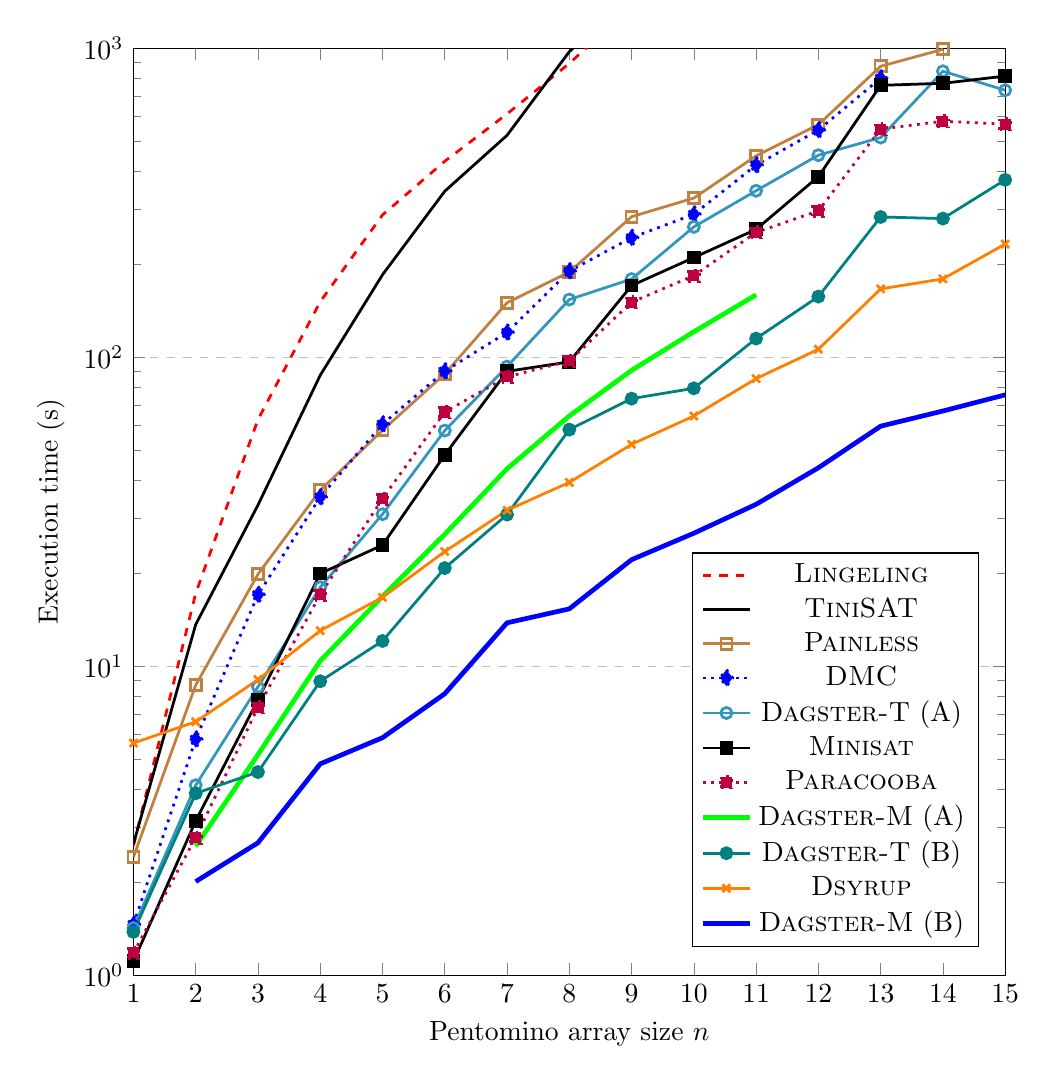
\begin{tikzpicture}
		\begin{axis}[
			title={},
			xlabel={Pentomino array size $n$},
			ylabel={Execution time (s)},
			xmin=1, xmax=15,
			ymin=1.00, ymax=1000.00,
			ymode=log,
			xtick={1,2,3,4,5,6,7,8,9,10,11,12,13,14,15},
			%ytick={0,20,40,60,80,100},
			%yticklabel=$\pgfmathprintnumber{\tick}\%$,
			legend pos=south east,
			ymajorgrids=true,
			grid style=dashed,
			xticklabel style={/pgf/number format/fixed},
			width = 360, %350,
			height = 380 %350 %260
		]


\addplot[color=red,line width=1.0pt,dashed] coordinates {
(1,2.626594543)(2,17.20426822)(3,62.83456993)(4,151.1784186)(5,288.6084802)(6,430.5156553)(7,612.4651904)(8,892.3813566)(9,1367.4057105)
}node[pos=0.8](endofplotsquare){} ;
\addlegendentry{\lingeling}

\addplot[color=black,line width=1.0pt] coordinates {
(1,2.65920496)(2,13.64072895)(3,33.22629547)(4,87.40588522)(5,184.7756422)(6,344.4516697)(7,522.2698565)(8,973.96888805)(9,1498.1676295)
}node[pos=0.8](endofplotsquare){} ;
\addlegendentry{\tinisat}

%\addplot[color=blue,line width=1.0pt] coordinates {
%(1,2.296598196029663)(2,5.464817523956299)(3,14.249489307403564)(4,32.19265341758728)(5,67.76493430137634)(6,159.12207126617432)(7,288.40518498420715)(8,480.1812901496887)(9,846.199215888977)(10,1108.5261766910553)(11,1689.7399978637695)(12,2593.415327310562)
%}node[pos=0.8](endofplotsquare){} ;
%\addlegendentry{\textsc{Painless} 10 cores}






\addplot[mark=square, color=brown,line width=1.0pt] coordinates {
(1, 2.41045880317688)
(2, 8.687188148498535)
(3, 19.8475661277771)
(4, 37.08610701560974)
(5, 58.00256848335266)
(6, 88.28625059127808)
(7, 150.01591539382935)
(8, 188.60771346092224)
(9, 284.8128137588501)
(10, 327.23674392700195)
(11, 448.22342324256897)
(12, 565.4391100406647)
(13, 873.8017907142639)
(14, 991.3404622077942)
}node[pos=0.8](endofplotsquare){} ;
\addlegendentry{\textsc{Painless} %17 cores
}








\addplot[mark=diamond*, mark options={scale=1.5}, color=blue,line width=1.0pt,dotted] coordinates {
(1, 1.46008515358)
(2, 5.8006169796)
(3, 17.0401728153)
(4, 35.2519440651)
(5, 60.7080829144)
(6, 90.0958409309)
(7, 120.235812187)
(8, 189.874330997)
(9, 243.533018112)
(10, 289.968929052)
(11, 418.34883654099997)
(12, 543.3793399333954)
(13, 799.2486734390259)
}node[pos=0.8](endofplotsquare){} ;
\addlegendentry{\textsc{DMC} %17 cores
}







\addplot[mark=o, color=black!25!cyan,line width=1.0pt] coordinates {
(1,1.4220540523529053)(2,4.118811130523682)(3,8.575927138328552)(4,18.005908012390137)(5,31.03825616836548)(6,57.88598895072937)(7,93.26125991344452)(8,153.65379166603088)(9,178.95973658561707)(10,264.0238370895386)(11,345.57388615608215)(12,450.41467809677124)(13,513.6661465167999)(14,841.9208600521088)(15,730.966267824173)
}node[pos=0.8](endofplotsquare){} ;
\addlegendentry{\textsc{Dagster-T} %17 cores
(A)}








\addplot[mark=square*,color=black,line width=1.0pt] coordinates {
(1, 1.1087782382965088)
(2, 3.158078193664551)
(3, 7.792155027389526)
(4, 19.9410183429718)
(5, 24.656651973724365)
(6, 48.2756884098053)
(7, 89.96435046195984)
(8, 96.55569005012512)
(9, 170.49162936210632)
(10, 210.04739713668823)
(11, 259.19717621803284)
(12, 383.92896032333374)
(13, 758.1628351211548)
(14, 769.5907070636749)
(15, 812.0646715164185)
}node[pos=0.8](endofplotsquare){} ;
\addlegendentry{\textsc{Minisat}}








\addplot[mark=square*, color=purple,line width=1.0pt,dotted] coordinates {
%(2, 2.8006629943847656)
%(3, 7.414581537246704)
%(4, 17.744986295700073)
%(5, 30.109254121780396)
%(6, 68.4067063331604)
%(7, 81.76717758178711)
%(8, 103.51843452453613)
%(9, 169.03482842445374)
%(10, 209.98187828063965)
%(11, 322.2795420885086)

(1, 1.1814595460891724)
(2, 2.7884726524353027)
(3, 7.364444255828857)
(4, 17.026161432266235)
(5, 34.85879373550415)
(6, 66.46172499656677)
(7, 86.3424642086029)
(8, 97.22442531585693)
(9, 150.61685132980347)
(10, 183.6677143573761)
(11, 253.38315439224243)
(12, 297.50710916519165)
(13, 547.255628824234)
(14, 579.9135086536407)
(15, 567.9678329229355)
}node[pos=0.8](endofplotsquare){} ;
\addlegendentry{\textsc{Paracooba} %17 cores
}




%\addplot[mark=*, color=teal,line width=1.0pt] coordinates {
%(1, 1.1411421298980713)
%(2, 3.7037432193756104)
%(3, 4.804152250289917)
%(4, 11.650121212005615)
%(5, 15.919332265853882)
%(6, 21.370890617370605)
%(7, 34.12385416030884)
%(8, 53.48321008682251)
%(9, 66.5775454044342)
%(10, 80.2962257862091)
%(11, 102.16768884658813)
%(12, 166.28865265846252)
%(13, 216.8384714126587)
%(14, 276.4749050140381)
%(15, 327.715101480484)
%}node[pos=0.8](endofplotsquare){} ;
%\addlegendentry{\dagster 17 cores (B) - no file loading}









\addplot[color=green,line width=1.7pt] coordinates {
(2, 2.6128995418548584)
(3, 5.1764607429504395)
(4, 10.406907081604004)
(5, 16.81988525390625)
(6, 26.716357469558716)
(7, 43.539146184921265)
(8, 64.54451870918274)
(9, 90.63454985618591)
(10, 120.82121872901917)
(11, 159.1339123249054)
}node[pos=0.8](endofplotsquare){} ;
\addlegendentry{\textsc{Dagster-M} %17 cores 
(A)}






\addplot[mark=*, color=teal,line width=1.0pt] coordinates {
(1, 1.3805564641952515)
(2, 3.878322124481201)
(3, 4.544595003128052)
(4, 8.937270641326904)
(5, 12.06746792793274)
(6, 20.770857572555542)
(7, 30.946043968200684)
(8, 58.292418479919434)
(9, 73.42058563232422)
(10, 79.31028938293457)
(11, 114.87923336029053)
(12, 157.0616569519043)
(13, 284.2289674282074)
(14, 280.90935039520264)
(15, 374.9265949726105)

}node[pos=0.8](endofplotsquare){} ;
\addlegendentry{\textsc{Dagster-T} %17 cores
(B)}








\addplot[mark=x, color=orange,line width=1.0pt] coordinates {
(1, 5.640398740768433)
(2, 6.608943462371826)
(3, 9.045408010482788)
(4, 13.032437562942505)
(5, 16.704758167266846)
(6, 23.499578952789307)
(7, 31.948850631713867)
(8, 39.34085011482239)
(9, 52.23883390426636)
(10, 64.5127785205841)
(11, 85.23249292373657)
(12, 106.06900763511658)
(13, 166.28967237472534)
(14, 179.21279311180115)
(15, 232.2783226966858)
}node[pos=0.8](endofplotsquare){} ;
\addlegendentry{\textsc{Dsyrup}% 17 cores
}






%\addplot[mark=square*,color=black,line width=1.7pt] coordinates {
%(2, 2.295314311981201)
%(3, 5.917216777801514)
%(4, 13.631609678268433)
%(5, 21.01494526863098)
%(6, 38.926801681518555)
%(7, 75.30455613136292)
%(8, 91.85509204864502)
%(9, 160.555278301239)
%(10, 190.86587381362915)
%(11, 270.93441796302795)
%(12, 360.38334226608276)
%(13, 541.1463418006897)
%(14, 644.4995956420898)
%(15, 807.9005448818207)
%}node[pos=0.8](endofplotsquare){} ;
%\addlegendentry{\textsc{Glucose-Syrup}}











\addplot[color=blue,line width=1.7pt] coordinates {
(2, 2.0096540451049805)
(3, 2.6825554370880127)
(4, 4.83022403717041)
(5, 5.869507312774658)
(6, 8.143877983093262)
(7, 13.815000772476196)
(8, 15.32940673828125)
(9, 22.113656759262085)
(10, 26.93359684944153)
(11, 33.40736651420593)
(12, 43.85346245765686)
(13, 59.806533336639404)
(14, 66.95989322662354)
(15, 75.51651453971863)
}node[pos=0.8](endofplotsquare){} ;
\addlegendentry{\textsc{Dagster-M} %17 cores
(B)}







		\end{axis}
		\end{tikzpicture}
		%\vspace{-18pt}
		\caption[Runtime performance for Pentomino problems]{Runtime model counting performance (medians across 86 samples) of \dagster\ (w/ decompositions A and B, w/ \tinisat\ (T) and \textsc{Minisat} (M) cores) against \tinisat, \lingeling, \textsc{Minisat}, \textsc{Painless-Mcomsps}, \textsc{Paracooba}, \textsc{DMC} and \textsc{Dsyrup} solvers, for $n\times n$ arrays of $15\times 15$ pentomino subproblems. all paralell algorithms use 17 cores.}
		\label{fig:performance_graph46461}
    \end{figure}

%   \begin{figure}[]
        \centering
		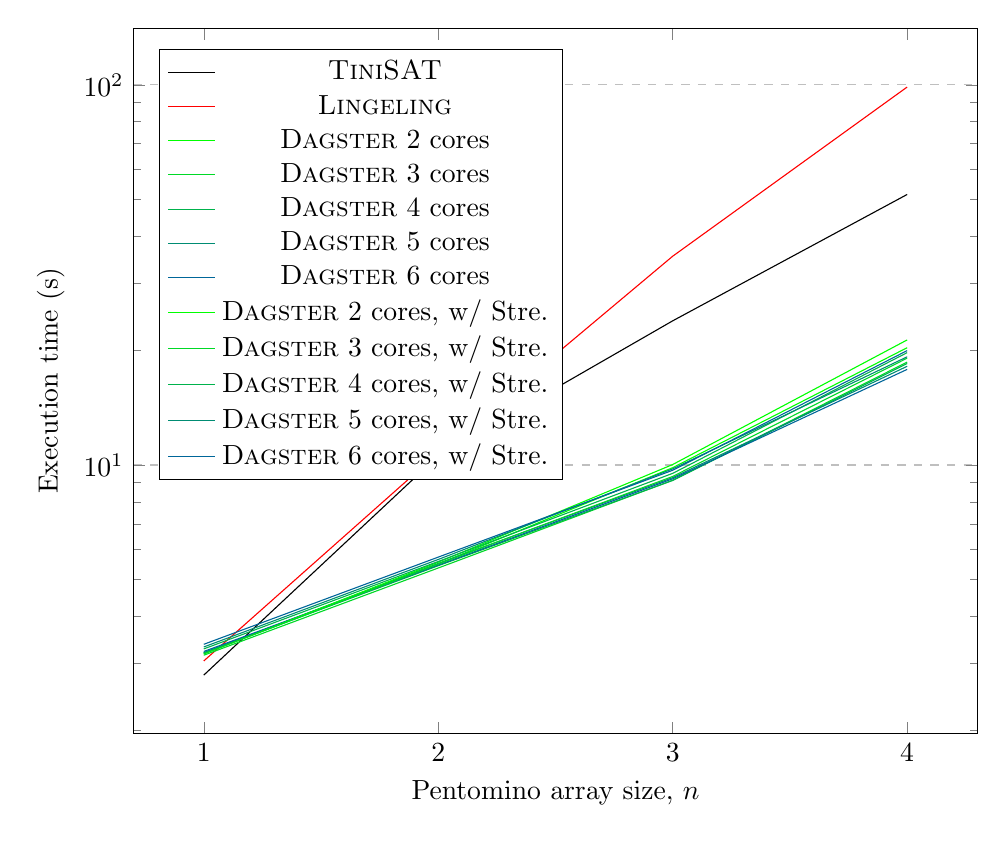
\begin{tikzpicture}
		\begin{axis}[
			title={},
			xlabel={Pentomino array size, $n$},
			ylabel={Execution time (s)},
			%xmin=0, xmax=0.25,
			%ymin=10.00, ymax=100000.00,
			ymode=log,
			xtick={1,2,3,4},
			%ytick={0,20,40,60,80,100},
			%yticklabel=$\pgfmathprintnumber{\tick}\%$,
			legend pos=north west,
			ymajorgrids=true,
			grid style=dashed,
			xticklabel style={/pgf/number format/fixed},
			width = 350,
			height = 300
		]


\addplot[color=black,line width=0.4pt] coordinates {
(1,2.80105912685394)(2,10.57788002491)(3,23.9460713863373)(4,51.4822851419449)
}node[pos=0.8](endofplotsquare){} ;
\addlegendentry{\tinisat}
\addplot[color=red,line width=0.4pt] coordinates {
(1,3.05225157737732)(2,10.7639915943146)(3,35.4204362630844)(4,98.6813420057297)
}node[pos=0.8](endofplotsquare){} ;
\addlegendentry{\lingeling}

\addplot[color=blue!0!green,line width=0.4pt] coordinates {
(1,3.20242965221405)(2,5.49430537223816)(3,9.83862674236298)(4,20.3514490127563)
}node[pos=0.8](endofplotsquare){} ;
\addlegendentry{\dagster 2 cores}
\addplot[color=blue!15!green,line width=0.4pt] coordinates {
(1,3.15934991836548)(2,5.35892224311829)(3,9.11750507354736)(4,18.654797077179)
}node[pos=0.8](endofplotsquare){} ;
\addlegendentry{\dagster 3 cores}
\addplot[color=blue!30!green,line width=0.4pt] coordinates {
(1,3.20555901527405)(2,5.43349432945251)(3,9.10745751857758)(4,18.4888120889664)
}node[pos=0.8](endofplotsquare){} ;
\addlegendentry{\dagster 4 cores}
\addplot[color=blue!45!green,line width=0.4pt] coordinates {
(1,3.20880806446075)(2,5.50885105133057)(3,9.26280069351196)(4,18.1849012374878)
}node[pos=0.8](endofplotsquare){} ;
\addlegendentry{\dagster 5 cores}
\addplot[color=blue!60!green,line width=0.4pt] coordinates {
(1,3.23214876651764)(2,5.45397925376892)(3,9.19934237003326)(4,17.846045255661)
}node[pos=0.8](endofplotsquare){} ;
\addlegendentry{\dagster 6 cores}




\addplot[color=blue!0!green,line width=0.4pt] coordinates {
(1,3.18395233154297)(2,5.55072700977325)(3,10.0285331010819)(4,21.3312681913376)
}node[pos=0.8](endofplotsquare){} ;
\addlegendentry{\dagster 2 cores, w/ Stre.}
\addplot[color=blue!15!green,line width=0.4pt] coordinates {
(1,3.18648815155029)(2,5.48706614971161)(3,9.33053779602051)(4,19.1051753759384)
}node[pos=0.8](endofplotsquare){} ;
\addlegendentry{\dagster 3 cores, w/ Stre.}
\addplot[color=blue!30!green,line width=0.4pt] coordinates {
(1,3.28249680995941)(2,5.57455515861511)(3,9.50650572776794)(4,19.7531452178955)
}node[pos=0.8](endofplotsquare){} ;
\addlegendentry{\dagster 4 cores, w/ Stre.}
\addplot[color=blue!45!green,line width=0.4pt] coordinates {
(1,3.3218799829483)(2,5.64312767982483)(3,9.76925492286682)(4,19.2610232830048)
}node[pos=0.8](endofplotsquare){} ;
\addlegendentry{\dagster 5 cores, w/ Stre.}
\addplot[color=blue!60!green,line width=0.4pt] coordinates {
(1,3.37587356567383)(2,5.72409021854401)(3,9.68606567382813)(4,19.9980112314224)
}node[pos=0.8](endofplotsquare){} ;
\addlegendentry{\dagster 6 cores, w/ Stre.}




		\end{axis}
		\end{tikzpicture}
		%\vspace{-18pt}
		\caption[Runtime performance for Pentomino problems with and without strengthener]{Runtime performance (specifically medians) of \dagster\ against \tinisat\ and \lingeling\ solvers for different numbers of cores, across $n$, for $n\times n$ grid of $15\times 15$ pentomino problems, with and without additional strengthening cores.}
		\label{fig:performance_graph4646ddd1}
    \end{figure}

%\input{figs/pentomino_memory_graph.tex}


\FloatBarrier
\pagebreak
\subsection{Bounded Model Checking with Abstraction Invariants}\label{sec:mc:bmc}

\paragraph{The New feature} of \dagster\ that is is used when generating the experimental data reported on for this case study is the sound and complete approach to trimming solution literals described in Section~\ref{sec:literal_trimming}. $\qed$\\\rule{50pt}{5pt}


We now describe a model checking case study, showing how \dagster\ can be used with existing tools to interrogate the functioning of finite-state-machines and circuits, and in particular to verify that a particular error state of the machine can be reached.
Our checking processes will be based on search performed by SAT reasoning, as exemplified in~\cite{DBLP:journals/ac/BiereCCSZ03}.
A survey of approaches to model checking software systems is in~\cite{SurveySymExec-CSUR18}, and we note a wide range of systems exist in this setting, including \textsc{CBMC} \cite{DBLP:conf/tacas/ClarkeKL04,10.1007/978-3-642-54862-8_26}, \textsc{F-Soft} \cite{DBLP:journals/tcs/IvancicYGGA08}, \textsc{ESBMC} \cite{DBLP:journals/tse/CordeiroFM12}, \textsc{LLBMC} \cite{DBLP:conf/kbse/FalkeMS13}, and \textsc{ESBMC} \cite{10.1007/s10009-020-00571-2}.
In our case study, we shall be using \textsc{CBMC} as the basis for generating structured SAT queries for \dagster. 
%%In this paper we consider CMBC bounded model checking software as a means of generating SAT queries for falsifying a specific communication protocol.

\newcommand{\pp}[1]{\ensuremath{\textsf{#1}}}

Our case study considers the wireless security protocol for communication with a implantable low-power medical device described in~\cite{5759785}. %{\em Alwen Tiu} 
{\em Alwen Tiu} determined {\em a priori} and by manual inspection that this protocol has a potential issue.
The protocol is based on encrypted communication using a 32bit secret key $K$, shared between an implantable medical device (IMD) and a base-station (BASE).
The IMD has a 32bit serial number $S$ that uniquely identifies it among other devices.
Both the IMD and BASE have a 32bit message counter,  $A$ for the devise, and $B$ for BASE, with both counters initially set to zero.
We use notation $X\&Y$ to denote bit string concatenation, and $\pp{Split}(A)$ to denote splitting a bit string A into two halves, and $\pp{Interleave}(A,B)$ to denote the result of interleaving $A$ and $B$ bit strings.
We also write $\{A\}_K$ to denote the bit string $A$ encrypted with $K$. For a message transmitted from the BASE to the IMD, and be accepted (i.e., not "dropped"), the following is required:

\begin{enumerate}
    \item BASE has a 64bit message $X$ (larger messages either chunked and/or padded into 64bits)
    \item BASE adds one to its message counter $B$
    \item BASE produces a message\\ $M_1,M_2=\pp{Split}(\pp{Interleave}(X,S\&B))$
    \item BASE sends the message $\{M_1\}_K\&\{M_2\}_K$ to IMD
    \item IMD receives $\{M_1\}_K\&\{M_2\}_K$ and decrypts each part with $K$ then joins and de-interleaves to find $X,S,B$
    \item IMD checks compatible $S$, if not match then drop message, it then checks message counter $B$ against its own counter $A$. If $B>A$ it accepts the message and sets $A$ to be equal to $B$, otherwise it drops the message
\end{enumerate}

From examining this protocol, we note there is a weakness. Particularly, an adversary can witnesses a message $\{M_1\}_K\&\{M_2\}_K$ from the BASE to the IMD, and then subsequently send a message $\{M_1\}_K\&\{M_1\}_K$ to the IMD. This message from the adversary will then causing the IMD's message counter $A$ to be incremented to $S$ (perhaps a large number), consequently causing the IMD to cease accepting legitimate messages from the BASE.
This error state in the protocol is subject to model checking, which can be done using \dagster.

We approach model checking this protocol compositionally, using \dagster, by appealing to a notion of process abstraction. 
Specifically, intending to proceed with \textsc{CBMC}, we faithfully describe the protocol in the C programming language. 
State variables describing the evolution of the protocol--e.g., whether an attacker or BASE is sending a message at timestep $i$---are of a fixed type. Variables encoding protocol registers, such as $A$, $B$, $X$, etc., being of a range of types, depending on where we are in an abstraction hierarchy. 
State variables of a fixed type we call {\em abstraction invariant} (AI).
Our abstraction hierarchy then considers the other variables at a range of fidelities, with 8-bit registers modelling protocol instructions at the highest level of abstraction (lowest fidelity) and 64-bit registers at the lowest level (highest fidelity).
We see that the protocol is much easier to model check, in practice, at a high abstraction level, and so our approach takes assignments to AI variables from satisfying assignments to highly abstract models, and uses those to inform search at lower levels of abstraction.  
%%
A simulated run of the bidirectional communication from the base-station (BASE) to the medical-device (IMD) was written in C programming for different fidelities of their variables, and passed to the CBMC software to generate corresponding SAT instance problems with annotations for AI variables' bit values.\footnote{%Anonymous submission, link to sources to be given if accepted.} 
Sourcecode:\\ \url{https://github.com/ThomWillingham/bmc-summer2122}}


We use \textsc{CBMC} to generate CNF representations of the protocol at different fidelities, producing annotated formulae that identify AI variables and the relationships between AI variables in different fidelity models. 
\dagster\ is used to automate the workflow, of solving the lower fidelity problem/s and then carrying across the AI variable values as constraints to the higher fidelity models - as indicated in the DAG shown in Figure \ref{fig:bmc_dag}.
%%
Here, we document the observed improvement in performance of this process, over running the higher fidelity models directly in a SAT solver. Our results are in Figure \ref{fig:performance_EMD}, where we can see that solving the 64 bit model using AI solutions from lower fidelity models results in a improvement in search performance.
%%
Particularly, in Figure~\ref{fig:performance_EMD} we can see that using AI variable information saves an order of magnitude on the number of conflicts encountered as well as a reduction of $\sim$5 times fewer variable assignments required.
%%
In this way AI information can be used to accelerate bounded model checking. The results presented here were achieved using \dagster\ in mode \modezero, with one CDCL \tinisat\ core.

\begin{figure}[]
\centering


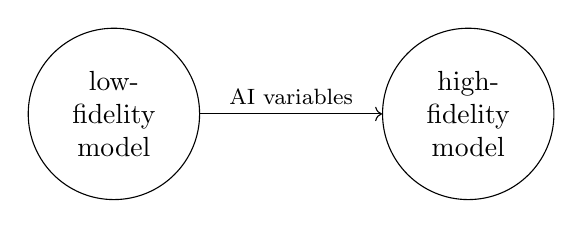
\begin{tikzpicture}[scale=0.9]
	\node [fill=white, draw=black, shape=circle, text width=1.5cm, text centered] (0) at (0, 0) {low-fidelity model};
	\node [fill=white, draw=black, shape=circle, text width=1.5cm, text centered] (1) at (5, 0) {high-fidelity model};
	\draw [fill=none, ->] (0) to node[above,pos=0.5]{\footnotesize AI variables} (1);
\end{tikzpicture}
%\caption{DAG for Costas problem.}\label{fig:dag_example121}





\caption[DAG for bounded model checking problem]{DAG for bounded model checking problem, showing AI variables being passed from the solution of low fidelity model to higher fidelity model}\label{fig:bmc_dag}
\end{figure}






\definecolor{bblue}{HTML}{4F81BD}
\definecolor{rred}{HTML}{C0504D}
\definecolor{ggreen}{HTML}{9BBB59}
\definecolor{ppurple}{HTML}{9F4C7C}

\begin{figure}
\begin{tikzpicture}
    \begin{axis}[
        width  = 0.8*\textwidth,
        height = 8cm,
        major x tick style = transparent,
        ybar=2*\pgflinewidth,
        bar width=14pt,
        ymajorgrids = true,
        %ylabel = {Run time speed},
        symbolic x coords={8 to 64,16 to 64,32 to 64,64},
        xtick = data,
        scaled y ticks = false,
        enlarge x limits=0.25,
        ymin=0,
		%	legend pos=south east,
        legend cell align=left,
        legend style={
                at={(1.05,0)},
                anchor=south west,
                column sep=1ex
        },
			ymode=log
    ]
        \addplot[style={bblue,fill=bblue,mark=none}]
            coordinates {(8 to 64, 19510) (16 to 64,22572) (32 to 64,29965) (64,21155)};

        \addplot[style={rred,fill=rred,mark=none}]
             coordinates {(8 to 64,204886) (16 to 64,206391) (32 to 64,470801) (64,636041)};

        \addplot[style={ggreen,fill=ggreen,mark=none}]
             coordinates {(8 to 64,77) (16 to 64,140) (32 to 64,457) (64,418)};


        \legend{decisions,variable assignments,conflicts}
    \end{axis}
\end{tikzpicture}
\caption[EMD model checking performance graph]{The SAT performance of EMD model checking with propagation AIs between different fidelities of the problem, between 8/16/32 bit instances and the 64 bit instance, with the 64 bit instance without propagation for comparison}\label{fig:performance_EMD}
\end{figure}


\section{Conclusions and Future Work}


We have outlined our new tool, \dagster, summarising some capabilities using two case studies: Costas arrays and pentomino tiling problems, and also demonstrating its use in bounded model checking.
The \dagster\ tool implements a number of search-based solution procedures for the Boolean SAT problem, including both systematic and local search procedures.
These have been integrated to operate in tandem, as a parallel hybrid search.
The \dagster\ tool takes as input a Boolean SAT problem, and a schematic description of the compositional structure of the SAT.
The tool operates in an HPC environment, and  distributes the search effort to solve the given problem according to the provided compositional structure.
It is able to operate on very large problems, and has been shown to accelerate Boolean SAT queries and model counting on a number of scenarios.
We have outlined a range of new features of the \dagster\ system since the last report deliverable.
We plan to support the continued development and expanded the features of the tool.

\FloatBarrier

\pagebreak
\renewcommand{\refname}{\spacedlowsmallcaps{References}} % For modifying the bibliography heading
\bibliographystyle{unsrt}
\bibliography{bib.bib} % The file containing the bibliography
\end{document}
